\documentclass[11pt,oneside]{article}

\usepackage[a4paper,margin=25mm,headheight=15pt]{geometry}
\usepackage[T1]{fontenc}
\usepackage[utf8]{inputenc}
\IfFileExists{libertinus.sty}{\usepackage{libertinus}}{\usepackage{lmodern}}
\usepackage{microtype}
\usepackage{amsmath,amssymb,amsthm,mathtools,mathrsfs,bm}
\usepackage{booktabs,longtable,tabularx,array,multirow}
\usepackage{graphicx}
\usepackage{caption}
\usepackage{float}
\usepackage{xcolor}
\usepackage{enumitem}
\usepackage{listings}
\usepackage{xurl}
\usepackage{fancyhdr}
\usepackage{titlesec}
\usepackage[hypertexnames=false]{hyperref}
\usepackage[nameinlink,noabbrev]{cleveref}
\usepackage{aliascnt}

\graphicspath{{generated/}}
\definecolor{linkblue}{RGB}{31,78,121}
\definecolor{deepgreen}{RGB}{35,105,78}
\definecolor{shadegray}{RGB}{246,247,249}
\definecolor{rulegray}{RGB}{194,201,208}
\hypersetup{
  colorlinks=true,
  linkcolor=linkblue,
  citecolor=deepgreen,
  urlcolor=linkblue,
  pdftitle={Legendre--Rvachev Self-Reconstruction on [-1,1]},
  pdfauthor={Research report for Vladimir Reshetnikov's ProveIt project},
  pdfsubject={Finite shifted-up synthesis, orthogonal atom blocks, energy identities, and quarter-grid lifting},
  pdfkeywords={Fabius function, Rvachev up-function, Legendre polynomials, Strang--Fix, Bell polynomials, Bernoulli numbers, Thue--Morse, Lambert W}
}

\pagestyle{fancy}
\fancyhf{}
\fancyhead[L]{\small Legendre--Rvachev self-reconstruction}
\fancyhead[R]{\small\nouppercase{\leftmark}}
\fancyfoot[C]{\thepage}
\renewcommand{\headrulewidth}{0.4pt}
\titleformat{\section}{\Large\bfseries}{\thesection}{0.7em}{}
\titleformat{\subsection}{\large\bfseries}{\thesubsection}{0.7em}{}
\titleformat{\subsubsection}{\normalsize\bfseries}{\thesubsubsection}{0.7em}{}
\setcounter{secnumdepth}{3}
\setcounter{tocdepth}{2}
\setlist[itemize]{leftmargin=2em,itemsep=0.25em,topsep=0.4em}
\setlist[enumerate]{leftmargin=2.3em,itemsep=0.25em,topsep=0.4em}
\setlength{\emergencystretch}{3em}
\allowdisplaybreaks[2]
\numberwithin{equation}{section}

\lstdefinestyle{pythonstyle}{
  language=Python,
  basicstyle=\ttfamily\footnotesize,
  backgroundcolor=\color{shadegray},
  frame=single,
  rulecolor=\color{rulegray},
  columns=fullflexible,
  keepspaces=true,
  showstringspaces=false,
  breaklines=true,
  xleftmargin=0.7em,
  xrightmargin=0.7em,
  aboveskip=0.8em,
  belowskip=0.8em
}

\newtheorem{theorem}{Theorem}[section]
\newcommand{\newsharedtheorem}[2]{%
  \newaliascnt{#1}{theorem}%
  \newtheorem{#1}[#1]{#2}%
  \aliascntresetthe{#1}%
}
\newsharedtheorem{proposition}{Proposition}
\newsharedtheorem{lemma}{Lemma}
\newsharedtheorem{corollary}{Corollary}
\newsharedtheorem{identity}{Identity}
\newsharedtheorem{conjecture}{Conjecture}
\newsharedtheorem{problem}{Problem}
\theoremstyle{definition}
\newtheorem{definition}[theorem]{Definition}
\newtheorem{example}[theorem]{Example}
\newtheorem{algorithm}[theorem]{Algorithm}
\theoremstyle{remark}
\newtheorem{remark}[theorem]{Remark}

\newenvironment{statusbox}[1]{%
  \par\smallskip\noindent\begin{center}\begin{minipage}{0.94\textwidth}%
  \hrule\vspace{0.55em}\noindent\textbf{#1}\par\smallskip
}{%
  \vspace{0.55em}\hrule\end{minipage}\end{center}\smallskip
}

\newcommand{\R}{\mathbb R}
\newcommand{\C}{\mathbb C}
\newcommand{\Q}{\mathbb Q}
\newcommand{\N}{\mathbb N}
\newcommand{\Z}{\mathbb Z}
\newcommand{\E}{\mathbb E}
\newcommand{\dd}{\,\mathrm d}
\newcommand{\e}{\mathrm e}
\newcommand{\ii}{\mathrm i}
\newcommand{\upf}{\operatorname{up}}
\newcommand{\sincpi}{\operatorname{sinc}_{\pi}}
\newcommand{\MM}{\mathsf M}
\newcommand{\Dscr}{\mathscr D_u}
\newcommand{\PiE}{\Pi^{\mathrm e}}
\newcommand{\Span}{\operatorname{span}}
\newcommand{\supp}{\operatorname{supp}}
\newcommand{\rank}{\operatorname{rank}}
\newcommand{\diag}{\operatorname{diag}}
\newcommand{\tr}{\operatorname{tr}}
\newcommand{\norm}[1]{\left\lVert#1\right\rVert}
\newcommand{\abs}[1]{\left\lvert#1\right\rvert}
\newcommand{\floor}[1]{\left\lfloor#1\right\rfloor}
\newcommand{\ceil}[1]{\left\lceil#1\right\rceil}
\newcommand{\inner}[2]{\left\langle#1,#2\right\rangle}
\newcommand{\bigO}{\mathcal O}
\newcommand{\smallo}{o}
\newcommand{\vtwo}{\nu_2}
\newcommand{\one}{\mathbf 1}
\newcommand{\repo}{\nolinkurl{Analysis/FabiusFunction/docs}}
\DeclareMathOperator{\ord}{ord}
\DeclareMathOperator{\Res}{Res}

\title{\bfseries Legendre--Rvachev Self-Reconstruction on $[-1,1]$\\[0.45em]
\large Finite literal-shift synthesis, orthogonal atom blocks,\\
positive rational energy series, infinite sinc integrals,\\
and quarter-grid lifting identities}
\author{Research report for Vladimir Reshetnikov's \texttt{ProveIt} project}
\date{30 August 2026}

\begin{document}
\maketitle

\begin{abstract}
Let $u=\upf$ be Rvachev's even $C^\infty$ probability density supported on
$[-1,1]$.  The current \texttt{ProveIt} corpus contains two apparently opposite
constructions: every polynomial on a compact interval can be synthesized
exactly from finitely many translates of $u$, while $u$ itself has an absolutely
and uniformly convergent Fourier--Legendre expansion
$u=\sum_{n\ge0}u_nP_{2n}$.  Specializing the polynomial theorem gives, with
$Q_d=\MM(D)^{-1}P_d$,
\[
 P_d(x)=2^{-d}\sum_{|k|<2^{d+1}}
 Q_d(k/2^d)u(x-k/2^d),\qquad -1\le x\le1.
\]
For the even modes in the expansion this becomes a nested quarter-grid formula
with scale $m_n=4^n$.  Substitution closes the loop blockwise:
\[
 u(x)=\sum_{n=0}^{\infty}\frac{u_n}{4^n}
 \sum_{|k|<2\cdot4^n}Q_{2n}(k/4^n)u(x-k/4^n).
\]
The basic loop and its non-flattening obstruction are already present in a
recent repository report.  The main contribution here is the additional
structure exposed after closing it.

Each finite translate train is exactly the orthogonal mode $u_nP_{2n}$.
Consequently the self-reconstruction is an orthogonal decomposition into
finite cancellation blocks, with exact Pythagorean tails and a hierarchy of
Sturm--Liouville energies.  In particular, if
$A_2=\int_0^1F(x)^2\dd x$, then
\[
 A_2=\sum_{n=0}^{\infty}\frac{u_n^2}{4n+1}
 =\frac1{2\pi}\int_0^\infty
 \prod_{r=1}^{\infty}
 \left(\frac{\sin(t/2^r)}{t/2^r}\right)^2\dd t,
\]
a positive series with exact rational partial sums; numerically
$A_2\approx0.40443676798398526$.

The lattices $4^n\Z^{-1}$ are nested.  Comparing two admissible lattices gives
an explicit finite null train
\[
 \sum_{|k|<2rm}\bigl(1-r\one_{r\mid k}\bigr)
 Q(k/(rm))u(x-k/(rm))=0,
\]
and, for successive Legendre partial sums, an exact lifting law: the
coarse-to-fine coefficient update is the sum of a null-space gauge correction
and one new orthogonal Legendre detail.  Endpoint differentiation yields
finite identities for all endpoint jets, while evaluation at the center gives
an exact central-binomial dyadic sum rule.

Finally, combining the known factorial asymptotic of $Q_{2n}(0)$ with the
nonanalyticity of $u$ sharpens the existing non-flattening theorem.  If
$c_n^{(0)}=u_nQ_{2n}(0)/4^n$ is the repeated central-atom coefficient, then
\[
 \limsup_{n\to\infty}
 \frac{|c_n^{(0)}|^{1/n}}{n^2}=\frac1{\pi^2\e^2}.
\]
Thus the canonical atomwise coefficients are superexponential along a
subsequence even though the resulting orthogonal blocks tend rapidly to zero.
The archive includes exact rational verification, numerical coefficient scans,
all figures, and a fully commented standalone Python program.
\end{abstract}

\begin{statusbox}{Novelty and evidence boundary}
The Fourier product, probability model, rational moments, polynomial synthesis
theorem, Fourier--Legendre coefficients, basic finite Legendre atomization,
blockwise self-loop, fixed-scale partial sums, reciprocal-MGF pole asymptotics,
and the original non-flattening theorem are imported from the repository
snapshot \texttt{faa3a9b94ac0e71abdc53c36fdf428222e4d2a8c}.  The recursive
TeX tree was audited, with canonical consolidated sources close-read and
archived duplicates or superseded siblings cross-checked by path inventory and
targeted full-text searches.  Results labeled ``new here'' were not found in
that snapshot after searches for their defining formulas and terminology.
This is a corpus-relative novelty statement, not an assertion of worldwide
priority.  Conjectures are explicitly labeled; numerical evidence is never
used in place of a proof.
\end{statusbox}

\begin{statusbox}{Formal status: Legendre energy}
Editorial update (2026-08-29): at compiled source checkpoint
\texttt{ca66a1247}, the subsequent Lean module
\path{FabiusLegendreEnergy.lean} defines the polynomial-form blocks
$B_n=u_nP_{2n}$ and formalizes their complete orthogonality formula
\eqref{eq:block-orthogonality}, the coefficient Parseval identity
\eqref{eq:parseval-up}, the exact coefficient tail
\eqref{eq:exact-L2-tail}, and the real-variable Legendre equality
\eqref{eq:A2-legendre}.  Its public tail API includes both a
\texttt{HasSum} theorem and a \texttt{tsum} equality.
\end{statusbox}

\begin{statusbox}{Formal status: rational and Fourier energy}
At compiled source checkpoint \texttt{9d5f41c2c}, the further module
\path{FabiusLegendreRationalEnergy.lean} adds the three executable definitions
\path{canonicalRvachevLegendreCoefficientRat},
\path{fabiusSquareEnergyTermRat}, and
\path{fabiusSquareEnergyPartialSumRat}.  Its fifteen public theorems are
\path{canonicalRvachevLegendreCoefficientRat_cast},
\path{canonicalRvachevLegendreCoefficientRat_zero},
\path{fabiusSquareEnergyTermRat_cast},
\path{fabiusSquareEnergyTermRat_nonneg},
\path{fabiusSquareEnergyTermRat_zero},
\path{fabiusSquareEnergyPartialSumRat_cast},
\path{monotone_fabiusSquareEnergyPartialSumRat},
\path{fabiusSquareEnergyPartialSumRat_pos},
\path{fabiusSquareEnergyPartialSumRat_zero},
\path{fabiusSquareEnergyPartialSumRat_one},
\path{fabiusSquareEnergyPartialSumRat_two},
\path{fabiusSquareEnergyPartialSumRat_three},
\path{hasSum_fabiusSquareEnergy_ratCast},
\path{fabiusSquareEnergy_eq_tsum_ratCast}, and
\path{tendsto_fabiusSquareEnergyPartialSumRat_cast}.  They certify the report's
claim that every partial sum in \eqref{eq:A2-legendre} is a positive rational
number and that the sequence is monotone with real casts converging to $A_2$.
They also certify all four displayed values in \eqref{eq:A2-first}: $1/4$,
$7/18$, $3271/8100$, and $3246043/8037225$ at $N=0,1,2,3$, respectively.

At compiled source checkpoint \texttt{b9b240bc0}, the further module
\path{FabiusSquareEnergyFourier.lean} exports no definitions and exactly four
theorems:
\path{integral_norm_sq_rvachevFourier_eq_two_mul_fabiusSquareEnergy},
\path{fabiusSquareEnergy_eq_integral_Ioi_norm_sq_rvachevFourier},
\path{fabiusSquareEnergy_eq_integral_Ioi_tprod_sinc_sq}, and
\path{fabiusSquareEnergy_eq_scaled_integral_Ioi_tprod_sinc_sq}.  The first two
identify the full real-axis squared Fourier mass with $2A_2$ and the
positive-half-line mass with $A_2$.  The last two close exactly the
Fourier-product and infinite-sinc equalities \eqref{eq:A2-fourier} and
\eqref{eq:A2-sinc}, including the $1/(2\pi)$ normalization and the shift from
the zero-based product to the one-based product.
\end{statusbox}

\begin{statusbox}{Formal status: moment--Appell foundation}
At compiled source checkpoint \texttt{a3854643d}, the subsequent module
\path{RvachevMomentAppell.lean} exports six public definitions:
\path{rvachevRawMomentRat}, \path{rvachevReciprocalMomentRat},
\path{rvachevAppellPolynomialRat}, \path{rvachevAppellPolynomial}, and
\path{rvachevDeconvolvedPolynomial}, together with
\path{rvachevDeconvolutionLinearMap}.  Of its thirty public theorems, the
previously catalogued twenty-four are
\path{rvachevRawMomentRat_zero}, \path{rvachevRawMomentRat_even},
\path{rvachevRawMomentRat_odd}, \path{rvachevReciprocalMomentRat_zero},
\path{binomialConv_rvachevRawMomentRat_reciprocal},
\path{rvachevReciprocalMomentRat_eq_completeBellPolynomial},
\path{monic_rvachevAppellPolynomialRat},
\path{natDegree_rvachevAppellPolynomialRat},
\path{rvachevAppellPolynomial_eq_poly_cast},
\path{monic_rvachevAppellPolynomial},
\path{natDegree_rvachevAppellPolynomial},
\path{eval_rvachevAppellPolynomial_add},
\path{integral_pow_mul_rvachev_eq_rvachevRawMomentRat_cast},
\path{integral_eval_rvachevAppellPolynomial_add_mul_rvachev},
\path{rvachevDeconvolutionLinearMap_apply},
\path{rvachevDeconvolvedPolynomial_zero},
\path{rvachevDeconvolvedPolynomial_add},
\path{rvachevDeconvolvedPolynomial_smul},
\path{rvachevDeconvolvedPolynomial_finsetSum},
\path{rvachevDeconvolvedPolynomial_C_mul},
\path{rvachevDeconvolvedPolynomial_monomial},
\path{rvachevDeconvolvedPolynomial_X_pow},
\path{natDegree_rvachevDeconvolvedPolynomial_le}, and
\path{integral_eval_rvachevDeconvolvedPolynomial_add_mul_rvachev}.  They
formalize the full rational raw-moment sequence, its formal
binomial-convolution reciprocal and complete-Bell description, rational and
real monic Appell families of exact degree, and the polynomial smoothing
inverse used below as a real linear map preserving zero, addition, scalar
multiplication, finite sums, and constant-polynomial multiplication, with
explicit monomial and $X^n$ simplification laws into the Rvachev--Appell
family.  This
closes the formal coefficient content behind
\eqref{eq:beta-bell} and the operational polynomial-deconvolution content of
\eqref{eq:deconvolution}--\eqref{eq:appell}, but not the displayed analytic
reciprocal-MGF, differential-series, or Appell generating-function identities.
\end{statusbox}

\begin{statusbox}{Formal status: exact deconvolution triangularity}
At the same compiled checkpoint, the six further public theorems are
\path{coeff_rvachevDeconvolvedPolynomial_natDegree},
\path{natDegree_rvachevDeconvolvedPolynomial},
\path{leadingCoeff_rvachevDeconvolvedPolynomial},
\path{rvachevDeconvolvedPolynomial_eq_zero_iff},
\path{rvachevDeconvolutionLinearMap_injective}, and
\path{rvachevDeconvolvedPolynomial_injective}.  They prove that deconvolution
preserves the coefficient in the original natural degree, hence preserves
exact natural degree and leading coefficient.  Its kernel is trivial, and it
is injective both as the packaged real linear map and as the underlying raw
operation.
\end{statusbox}

\begin{statusbox}{Formal status: synthesis and translate blocks}
At compiled source checkpoint \texttt{a3854643d},
\path{RvachevPolynomialSynthesis.lean} exports no public definitions and
exactly four public theorems:
\path{tsum_rvachevDeconvolvedPolynomial_mul_shifted_rvachevUp},
\path{normalized_tsum_rvachevDeconvolvedPolynomial_mul_shifted_rvachevUp},
\path{sum_Ioo_rvachevDeconvolvedPolynomial_mul_shifted_rvachevUp}, and
\path{normalized_sum_Ioo_rvachevDeconvolvedPolynomial_mul_shifted_rvachevUp}.
They prove global raw and normalized \texttt{tsum} synthesis for every nonzero
natural mesh $m$ with \(\deg p\le\nu_2(m)\), and on $[-1,1]$ its exact finite
open-index form $-2m<k<2m$.  Thus the sufficient-condition and boxed-formula
content of \eqref{eq:generic-synthesis} is formalized.

At the same checkpoint, \path{FabiusLegendreTranslateBlocks.lean} exports six
public definitions: \path{rvachevLegendreDeconvolutionPolynomial},
\path{rvachevLegendreScale}, \path{rvachevLegendreIndexSet},
\path{rvachevLegendreAtomCoefficient},
\path{rvachevLegendreTranslateBlock}, and \path{rvachevTranslateGram}.  Its seven
public theorems are
\path{natDegree_rvachevLegendreDeconvolutionPolynomial},
\path{leadingCoeff_rvachevLegendreDeconvolutionPolynomial},
\path{eval_legendrePolynomial_eq_sum_rvachevUp},
\path{eval_legendrePolynomial_even_eq_sum_rvachevUp},
\path{rvachevLegendreTranslateBlock_eq_rvachevLegendreBlock},
\path{intervalIntegral_rvachevLegendreTranslateBlock_mul}, and
\path{sum_rvachevLegendreAtomCoefficient_mul_gram}.  They formalize the
deconvolved Legendre definition \eqref{eq:Q-def}, the finite formulas
\eqref{eq:Pd-synthesis} and \eqref{eq:even-P-synthesis}, the literal finite
block data and equality \eqref{eq:block-def}--\eqref{eq:block-mode}, complete
orthogonality of those translate blocks, and the atom-Gram identity
\eqref{eq:atom-gram}.  In addition, for $Q_d=\Dscr P_d$ they prove exact
degree $d$ and the explicit unchanged leading coefficient
$2^{-d}\binom{2d}{d}$.

\end{statusbox}
\begin{statusbox}{Formal status: universal composite-mesh sharpness}
Editorial update (2026-08-30): the focused-build module
\path{CompositeMeshSharpness.lean} exports one public definition,
\path{rvachevCombExactThrough}, and seven public theorems:
\path{exists_shift_tsum_shifted_monomial_ne_integral_nat_real},
\path{rvachevCombExactThrough_iff_padicValNat},
\path{rvachevCombExactThrough_iff_pow_two_dvd},
\path{rvachevCombExactThrough_two_pow},
\path{two_pow_le_of_rvachevCombExactThrough},
\path{isLeast_rvachevCombExactThrough}, and
\path{isLeast_rvachevCombExactThrough_even}.  Universal exactness means
exactness at every real shift for every real polynomial of natural degree at
most \(d\), with a nonzero natural mesh \(M\).  The classification is exactly
\(d\le\vtwo(M)\), equivalently \(2^d\mid M\); a monomial of degree
\(\vtwo(M)+1\) fails at some real shift; and \(2^d\) is the least universally
exact mesh.  The even-degree specialization makes \(4^N\) least for the
\emph{whole} polynomial space through degree \(2N\).  It does not assert
minimality for one Legendre polynomial, one fixed \(S_N\), or any
target-adapted mesh.
\end{statusbox}

\begin{statusbox}{Formal status: translate-block series and common-mesh convergence}

At compiled source checkpoint \texttt{a3854643d}, the focused-build module
\path{FabiusLegendreTranslateSeries.lean} exports five
public definitions:
\path{rvachevLegendrePartialSumDeconvolutionPolynomial},
\path{rvachevLegendrePartialSumAtomCoefficient},
\path{rvachevLegendrePartialSumTranslateBlock},
\path{rvachevLegendreTranslateBlockOnInterval}, and
\path{rvachevLegendrePartialSumTranslateBlockOnInterval}.  Its twenty-five public theorems
are
\path{natDegree_rvachevLegendrePartialSumDeconvolutionPolynomial},
\path{leadingCoeff_rvachevLegendrePartialSumDeconvolutionPolynomial},
\path{summable_norm_rvachevLegendreTranslateBlock},
\path{summable_rvachevLegendreTranslateBlock},
\path{hasSum_rvachevLegendreTranslateBlock},
\path{tsum_rvachevLegendreTranslateBlock},
\path{rvachevLegendrePartialSumDeconvolutionPolynomial_eq_sum},
\path{rvachevLegendrePartialSumAtomCoefficient_eq_sum},
\path{eval_rvachevLegendrePartialSumPolynomial_eq_tsum_rvachevUp},
\path{eval_rvachevLegendrePartialSumPolynomial_eq_sum_rvachevUp},
\path{rvachevLegendrePartialSumTranslateBlock_eq_eval_partialSumPolynomial},
\path{rvachevLegendrePartialSumTranslateBlock_eq_sum_translateBlock},
\path{rvachevLegendreTranslateBlockOnInterval_apply},
\path{rvachevLegendreTranslateBlockOnInterval_eq_smul},
\path{summable_norm_rvachevLegendreTranslateBlockOnInterval},
\path{summable_rvachevLegendreTranslateBlockOnInterval},
\path{hasSum_rvachevLegendreTranslateBlock_uniform},
\path{tsum_rvachevLegendreTranslateBlock_uniform},
\path{rvachevLegendrePartialSumTranslateBlockOnInterval_apply},
\path{rvachevLegendrePartialSumTranslateBlockOnInterval_eq_eval_partialSumPolynomial},
\path{rvachevLegendrePartialSumTranslateBlockOnInterval_eq_sum},
\path{tendsto_rvachevLegendrePartialSumTranslateBlockOnInterval},
\path{rvachevLegendrePartialSumTranslateBlock_tendstoUniformlyOn},
\path{tendsto_norm_rvachevLegendrePartialSumTranslateBlockOnInterval_sub}, and
\path{tendsto_rvachevLegendrePartialSumTranslateBlock}.
\end{statusbox}

\clearpage
\begin{statusbox}{Formal consequences and remaining boundary}
They close the pointwise
and uniform, absolutely summable literal-block loop
\eqref{eq:block-loop}; the full deconvolution identity \eqref{eq:SN-CN}; and
the global and finite common-mesh synthesis \eqref{eq:fixed-scale}.  They also
identify the named fixed-scale train with both the polynomial partial sum and
the sum of its separately scaled blocks as functions on $[-1,1]$.  The bundled
common-mesh partial trains converge to $u$ in $C([-1,1])$, equivalently in the
supremum norm, with raw \texttt{TendstoUniformlyOn}, norm-error-to-zero, and
pointwise forms also exposed.  The two new triangularity wrappers prove that
$C_N=\Dscr S_N$ has exactly the natural degree and leading coefficient of
$S_N$, including degenerate partial sums whose visible degree drops.

The universal-space API now proves the least natural mesh for the complete
degree-bounded polynomial space, but not minimality of the displayed mesh for
an individual \(P_d\), Legendre block, or particular \(S_N\).  The APIs still
do not prove reciprocal/deconvolution parity or the derivative, Gegenbauer,
Appell, and low-degree formulas for $Q_d$; rationality of the atom rows;
equality of the
fixed-scale and separately scaled coefficient vectors; an unconditional
$\operatorname{natDegree}(S_N)=2N$ theorem or nonvanishing of its top Legendre
coefficient; or the later refinement, projector, and asymptotic layers.
\end{statusbox}

At the recorded checkpoints, the public definition/theorem inventories of
\path{RvachevMomentAppell.lean}, \path{RvachevPolynomialSynthesis.lean},
\path{CompositeMeshSharpness.lean}, \path{FabiusLegendreTranslateBlocks.lean},
and \path{FabiusLegendreTranslateSeries.lean} are respectively $6/30$, $0/4$,
$1/7$, $6/7$, and $5/25$: exactly $91$ public declarations.

\clearpage
\tableofcontents
\clearpage

\section{Corpus audit and mathematical orientation}
\label{sec:audit}

\subsection{Principal repository inputs}

The relevant corpus is unusually rich and contains several reports answering
closely related prompts.  The following sources carry the load-bearing facts
used below.

\begin{longtable}{@{}p{0.34\textwidth}p{0.60\textwidth}@{}}
\toprule
\textbf{Repository source} & \textbf{Role in this report}\\
\midrule
\endfirsthead
\toprule
\textbf{Repository source} & \textbf{Role in this report}\\
\midrule
\endhead
{\footnotesize\nolinkurl{Fabius_Function_and_Rvachev_Up/}} &
Canonical normalization, Fourier product, moments, dyadic values, and the exact
Fourier--Legendre expansion with rational coefficients.\\
{\footnotesize\nolinkurl{Up_Polynomial_Synthesis/}} &
Consolidated exact reproduction of arbitrary polynomials by shifted or dilated
up-atoms; dyadic alias multiplicities; Bell--Bernoulli deconvolution; local
nullspaces and endpoint compression.\\
{\footnotesize\nolinkurl{lagrange_rvachev_loop_report_v3/}} &
The directly preceding Legendre-aware loop report: deconvolved Legendre
polynomials, Christoffel--Darboux synthesis, fixed-scale partial loops,
factorial growth of $Q_{2n}(0)$, and rigorous non-flattening.\\
The other four Lagrange--Rvachev loop siblings &
Independent checks of the same general finite synthesis, including exact
right-inverse calculations and oblique-projector conditioning.  They were
used as consistency checks rather than treated as five independent theorems.\\
Fourier-decay, inverse, Lambert-$W$, $q$-analog, and asymptotic reports &
Context for the sinc product, dyadic pole shells, lower/principal Lambert
branches, q-binomial formulas, and proposed asymptotics of endpoint and
spectral quantities.\\
\bottomrule
\end{longtable}

The recursive tree also contains historical versions, source copies inside
archives, and generated consolidation documents.  Counting every byte-distinct
copy as independent evidence would obscure rather than strengthen the audit.
The approach taken here was therefore: enumerate the full TeX tree, identify
canonical or newest representatives, compare neighboring reports, and search
the entire repository for the precise formulas introduced below.

\subsection{Imported, specialized, and new deductions}

\begin{table}[H]
\centering
\small
\begin{tabularx}{\textwidth}{@{}p{0.23\textwidth}X@{}}
\toprule
Status & Mathematical content\\
\midrule
Imported &
$\widehat u(\xi)=\prod_{j\ge0}\sincpi(\xi/2^j)$,
$\ord_{\xi=m}\widehat u=1+\vtwo(m)$, the MGF and cumulants, rational moments,
and exact dyadic values.\\
Imported &
Exact polynomial synthesis at any admissible dyadic oversampling ratio,
including the unit-radius literal-shift formula on $[-1,1]$.\\
Imported &
$u=\sum u_nP_{2n}$ with absolute and uniform convergence; exact rational
$u_n$; $Q_n=\Dscr P_n$; the basic block loop and fixed-scale partial loops.\\
Imported &
The factorial asymptotic of $Q_{2n}(0)$ and the theorem that the canonical loop
cannot be flattened into an absolute or unconditional atom series.\\
Specialized here &
A self-contained Legendre specialization for every $P_d$, including explicit
Bell--Bernoulli coefficient formulas, low-degree examples, and endpoint/center
sum rules.\\
New here, corpus-relative &
Orthogonality of the finite translate blocks, atom-Gram identities, exact
Pythagorean tails, rank-one atomized detail projectors, and the full
Sturm--Liouville energy hierarchy.\\
New here, corpus-relative &
The positive rational expansion and infinite-sinc integral for
$\int_0^1F^2$, together with a nested exact dyadic-Fabius square series.\\
New here, corpus-relative &
General interlevel null trains, the quarter-grid refinement cocycle, and an
exact lifting decomposition of successive fixed-scale coefficient vectors.\\
New here, corpus-relative &
Even-projector dual-frame trace identities and the sharp root-limsup law
$\limsup |c_n^{(0)}|^{1/n}/n^2=(\pi^2\e^2)^{-1}$.\\
\bottomrule
\end{tabularx}
\caption{Status of the principal results.}
\label{tab:status}
\end{table}

\section{Rvachev's atom, its MGF, and polynomial deconvolution}
\label{sec:foundations}

\subsection{Normalization and Fourier product}

Let $u=\upf$ be the unique even nonnegative $C^\infty$ function such that
\begin{equation}
 \supp u=[-1,1],\qquad u(0)=1,\qquad
 u'(x)=2u(2x+1)-2u(2x-1).
 \label{eq:up-dde}
\end{equation}
The chosen normalization also gives
\begin{equation}
 \int_{-1}^{1}u(x)\dd x=1.
 \label{eq:up-probability}
\end{equation}
With
\(
 \widehat f(\xi)=\int_{\R}f(x)e^{-2\pi\ii x\xi}\dd x
\),
\begin{equation}
 \widehat u(\xi)=
 \prod_{j=0}^{\infty}\sincpi(\xi/2^j),
 \qquad
 \sincpi(t)=\frac{\sin(\pi t)}{\pi t}.
 \label{eq:fourier-product}
\end{equation}
Every nonzero integer zero has the exact multiplicity
\begin{equation}
 \ord_{\xi=m}\widehat u(\xi)=1+\vtwo(m).
 \label{eq:zero-order}
\end{equation}
These multiplicities are the source of the sharp dyadic reproduction order.
They are also the Fourier shadow of the q-integer and Thue--Morse annihilators
appearing in local coefficient compression.

Equivalently, if $V_j$ are independent uniform random variables on $[-1,1]$,
then
\begin{equation}
 Z=\sum_{j=1}^{\infty}2^{-j}V_j
 \label{eq:random-series}
\end{equation}
has density $u$.  Hence the moment generating function is
\begin{equation}
 \MM(z)=\E e^{zZ}
 =\int_{-1}^{1}e^{zx}u(x)\dd x
 =\prod_{j=1}^{\infty}\frac{\sinh(z/2^j)}{z/2^j}.
 \label{eq:mgf}
\end{equation}

\subsection{Bernoulli cumulants and Bell-polynomial inverse}

Write
\begin{equation}
 \log\MM(z)=\sum_{r\ge1}\kappa_r\frac{z^r}{r!}.
 \label{eq:cumulant-def}
\end{equation}
Symmetry gives $\kappa_{2r+1}=0$, while
\begin{equation}
 \kappa_{2r}=\frac{B_{2r}}{2r(1-4^{-r})}
 =\frac{2^{2r-1}B_{2r}}{r(2^{2r}-1)}.
 \label{eq:cumulants}
\end{equation}
Define reciprocal coefficients by
\begin{equation}
 \frac1{\MM(z)}=\sum_{r=0}^{\infty}\beta_r\frac{z^r}{r!}.
 \label{eq:beta-def}
\end{equation}
Then $\beta_{2r+1}=0$ and, in complete Bell-polynomial notation,
\begin{equation}
 \beta_n=Y_n(-\kappa_1,-\kappa_2,\ldots,-\kappa_n).
 \label{eq:beta-bell}
\end{equation}
The first nonzero values are
\begin{equation}
 \beta_0=1,\qquad
 \beta_2=-\frac19,\qquad
 \beta_4=\frac{31}{675},\qquad
 \beta_6=-\frac{2347}{59535},\qquad
 \beta_8=\frac{1904369}{32531625}.
 \label{eq:beta-first}
\end{equation}

On polynomials the formal operator
\begin{equation}
 \Dscr:=\MM(D)^{-1}
 =\sum_{r\ge0}\beta_r\frac{D^r}{r!}
 \label{eq:deconvolution}
\end{equation}
terminates exactly.  It reverses convolution by the up probability law in the
polynomial category.  Its Appell sequence
\begin{equation}
 A_n(x)=\Dscr x^n,
 \qquad
 \frac{e^{xz}}{\MM(z)}=\sum_{n\ge0}A_n(x)\frac{z^n}{n!}
 \label{eq:appell}
\end{equation}
is therefore a finite Bell--Bernoulli coefficient engine for every synthesis
formula below.

\subsection{The imported exact polynomial theorem}

The unit-radius specialization of the repository's polynomial synthesis
result is the following.

\begin{theorem}[Exact literal-shift synthesis; imported]
\label{thm:generic-synthesis}
Let $p$ be a polynomial of degree at most $d$.  If $m\in\N$ satisfies
$\vtwo(m)\ge d$, put $p^\sharp=\Dscr p$.  Then, for $-1\le x\le1$,
\begin{equation}
 \boxed{
 p(x)=\frac1m\sum_{|k|<2m}p^\sharp(k/m)u(x-k/m).}
 \label{eq:generic-synthesis}
\end{equation}
The canonical minimal admissible ratio is $m=2^d$, giving $4m-1$ displayed
atoms.
\end{theorem}

\begin{proof}[Mechanism of proof]
Poisson summation converts the sampled translate train into a sum over Fourier
aliases.  At the zero alias, convolution by $u$ acts on polynomials as
$\MM(D)$, which is exactly inverted by $\Dscr$.  At every nonzero alias, the
zero multiplicity \eqref{eq:zero-order} is at least $d+1$, so all distributional
derivatives through degree $d$ vanish.  Compact support reduces the globally
locally finite train to the displayed finite range on $[-1,1]$.  The leading
coefficient of a degree-$d$ polynomial shows why the condition
$\vtwo(m)\ge d$ is sharp within this stationary Poisson-synthesis scheme.
\end{proof}

The focused-build declaration \path{isLeast_rvachevCombExactThrough} now
certifies the corresponding least-mesh statement when exactness is required
for \emph{every} polynomial of degree at most $d$ and every shift.  Its
classification companions are \path{rvachevCombExactThrough_iff_padicValNat}
and \path{rvachevCombExactThrough_iff_pow_two_dvd}.  This is the universal
whole-space reading of the last sentence of the theorem, not a
target-by-target minimality result.

\section{Finite shifted-up synthesis of Legendre polynomials}
\label{sec:legendre-synthesis}

\subsection{The deconvolved Legendre family}

Let $P_d$ be the Legendre polynomial normalized by $P_d(1)=1$, and define
\begin{equation}
 Q_d(x):=\Dscr P_d(x).
 \label{eq:Q-def}
\end{equation}
Because $\Dscr$ contains only even derivatives,
\begin{equation}
 Q_d(-x)=(-1)^dQ_d(x).
 \label{eq:Q-parity}
\end{equation}
There are several useful finite forms.  Directly from
\eqref{eq:deconvolution},
\begin{equation}
 Q_d(x)=\sum_{r=0}^{\floor{d/2}}
 \frac{\beta_{2r}}{(2r)!}P_d^{(2r)}(x).
 \label{eq:Q-derivative}
\end{equation}
Using
$P_d^{(2r)}=(4r-1)!!\,C_{d-2r}^{2r+1/2}$ gives
\begin{equation}
 Q_d(x)=\sum_{r=0}^{\floor{d/2}}
 \frac{\beta_{2r}(4r-1)!!}{(2r)!}
 C_{d-2r}^{2r+1/2}(x).
 \label{eq:Q-gegenbauer}
\end{equation}
Alternatively, applying $\Dscr x^j=A_j(x)$ to the standard power expansion,
\begin{equation}
 Q_d(x)=2^{-d}\sum_{r=0}^{\floor{d/2}}(-1)^r
 \frac{(2d-2r)!}{r!(d-r)!(d-2r)!}A_{d-2r}(x).
 \label{eq:Q-appell}
\end{equation}
Thus every coefficient is an explicit finite Bell polynomial in the Bernoulli
numbers.

The first members are
\begin{align}
 Q_0(x)&=1,\qquad Q_1(x)=x,\label{eq:Q01}\\
 Q_2(x)&=\frac32x^2-\frac23,\label{eq:Q2}\\
 Q_3(x)&=\frac52x^3-\frac73x,\label{eq:Q3}\\
 Q_4(x)&=\frac{35}{8}x^4-\frac{20}{3}x^2+\frac{134}{135},\label{eq:Q4}\\
 Q_5(x)&=\frac{63}{8}x^5-\frac{35}{2}x^3+\frac{33}{5}x,\label{eq:Q5}\\
 Q_6(x)&=\frac{231}{16}x^6-\frac{175}{4}x^4
        +\frac{889}{30}x^2-\frac{1426}{567}.
 \label{eq:Q6}
\end{align}
They are not orthogonal.  Their role is instead exact coefficient
preconditioning: $Q_d$ removes the moments introduced by the atom $u$.

\subsection{The requested finite Legendre representation}

\begin{theorem}[Finite shifted-up representation of $P_d$]
\label{thm:Pd-synthesis}
For every $d\ge0$, put $m_d=2^d$.  Then
\begin{equation}
 \boxed{
 P_d(x)=\frac1{2^d}
 \sum_{|k|<2^{d+1}}Q_d(k/2^d)u(x-k/2^d),
 \qquad -1\le x\le1.}
 \label{eq:Pd-synthesis}
\end{equation}
The formula has $2^{d+2}-1$ literal translates of the same, unscaled
up-function.  Within the stationary scheme of \cref{thm:generic-synthesis},
$m_d=2^d$ is minimal.
\end{theorem}

\begin{proof}
Apply \cref{thm:generic-synthesis} to $p=P_d$.  Its exact degree is $d$ and its
deconvolution is $Q_d$, so the canonical ratio is $m=2^d$.
\end{proof}

The first three cases are already informative.  On $[-1,1]$,
\begin{align}
 1&=u(x+1)+u(x)+u(x-1),
 \label{eq:P0-example}\\
 x&=\frac14\sum_{k=-3}^{3}k\,u(x-k/2),
 \label{eq:P1-example}\\
 P_2(x)&=\sum_{k=-7}^{7}
 \frac{9k^2-64}{384}\,u(x-k/4).
 \label{eq:P2-example}
\end{align}
The signs in \eqref{eq:P2-example} are indispensable: exact polynomial
reproduction is a cancellation identity, not a positive-mixture formula.

\subsection{Even modes and the nested quarter-grid}

For the modes that occur in the expansion of the even function $u$, set
\begin{equation}
 m_n:=2^{2n}=4^n.
 \label{eq:mn}
\end{equation}
Then \eqref{eq:Pd-synthesis} becomes
\begin{equation}
 \boxed{
 P_{2n}(x)=\frac1{4^n}
 \sum_{|k|<2\cdot4^n}Q_{2n}(k/4^n)u(x-k/4^n).}
 \label{eq:even-P-synthesis}
\end{equation}
The grids are nested:
\begin{equation}
 \frac1{m_n}\Z\subset\frac1{m_{n+1}}\Z,
 \qquad m_{n+1}=4m_n.
 \label{eq:nested-grids}
\end{equation}
This elementary observation is the seed of the exact multiresolution
identities in \cref{sec:nested}.

\section{Closing the existing Fourier--Legendre loop}
\label{sec:closing}

\subsection{Exact rational Legendre coefficients}

The canonical expansion in the repository is
\begin{equation}
 u(x)=\sum_{n=0}^{\infty}u_nP_{2n}(x),
 \qquad
 u_n=\frac{4n+1}{2}\int_{-1}^{1}u(x)P_{2n}(x)\dd x.
 \label{eq:legendre-series}
\end{equation}
It converges absolutely and uniformly on $[-1,1]$.  If
$\mu_{2j}=\int x^{2j}u(x)\dd x$, then
\begin{equation}
 u_n=\frac{4n+1}{2^{2n+1}}
 \sum_{j=0}^{n}(-1)^{n+j}
 \binom{2n}{n+j}\binom{2n+2j}{2n}\mu_{2j}.
 \label{eq:un-moments}
\end{equation}
The repository's dyadic moment bridge
\begin{equation}
 \mu_{2j}=2(2j)!\,2^{\binom{2j+1}{2}}F(2^{-2j-1})
 \label{eq:moment-fabius}
\end{equation}
makes every $u_n$ rational.  Combining the two equations gives
\begin{equation}
 u_n=4^{-n}(4n+1)\sum_{j=0}^{n}(-1)^{n+j}
 \binom{2n}{n+j}\binom{2n+2j}{2n}(2j)!
 2^{\binom{2j+1}{2}}F(2^{-2j-1}).
 \label{eq:un-dyadic}
\end{equation}

\begin{table}[H]
\centering
\small
\begin{tabular}{@{}rrrr@{}}
\toprule
$n$ & $u_n$ & $Q_{2n}(0)$ & $u_nQ_{2n}(0)/4^n$\\
\midrule
0 & $1/2$ & $1$ & $1/2$\\
1 & $-5/6$ & $-2/3$ & $5/36$\\
2 & $11/30$ & $134/135$ & $737/32400$\\
3 & $143/5670$ & $-1426/567$ & $-101959/102876480$\\
4 & $-7291/85050$ & $7587914/722925$ & $-0.00351481095499\ldots$\\
5 & $99137/2485890$ & $-9200178166/130509225$ & $-0.00274542090064\ldots$\\
6 & $-5726162257/213774110550$ & $728.294733513\ldots$ & $-0.00476272782254\ldots$\\
\bottomrule
\end{tabular}
\caption{First Legendre, deconvolution, and central-atom coefficients.  Exact
fractions for all displayed decimals are in the accompanying CSV file.}
\label{tab:first-coefficients}
\end{table}

\subsection{The blockwise self-loop}

Substituting \eqref{eq:even-P-synthesis} into
\eqref{eq:legendre-series} yields the exact loop already established in the
recent Legendre-aware repository report.

\begin{theorem}[Blockwise Legendre--Rvachev loop; imported]
\label{thm:block-loop}
Define
\begin{equation}
 B_n(x):=\frac{u_n}{m_n}
 \sum_{|k|<2m_n}Q_{2n}(k/m_n)u(x-k/m_n).
 \label{eq:block-def}
\end{equation}
Then, on $[-1,1]$,
\begin{equation}
 B_n(x)=u_nP_{2n}(x),
 \label{eq:block-mode}
\end{equation}
and
\begin{equation}
 \boxed{u(x)=\sum_{n=0}^{\infty}B_n(x).}
 \label{eq:block-loop}
\end{equation}
The outer series converges absolutely and uniformly when every finite inner
train is retained as one block.
\end{theorem}

\begin{proof}
Equation \eqref{eq:block-mode} is
\eqref{eq:even-P-synthesis} multiplied by $u_n$.  Since
$\norm{P_j}_{L^\infty[-1,1]}\le1$ and the imported expansion satisfies
$\sum|u_n|<\infty$, the Weierstrass test proves the stated block convergence.
\end{proof}

The focused-build declarations
\path{summable_norm_rvachevLegendreTranslateBlock},
\path{hasSum_rvachevLegendreTranslateBlock}, and
\path{tsum_rvachevLegendreTranslateBlock} certify the literal pointwise
series.  Their continuous-map counterparts
\path{summable_norm_rvachevLegendreTranslateBlockOnInterval},
\path{hasSum_rvachevLegendreTranslateBlock_uniform}, and
\path{tsum_rvachevLegendreTranslateBlock_uniform} certify the absolute
supremum-norm bound and uniform sum on the whole interval.  Thus the full
statement of \cref{thm:block-loop}, with each inner train kept as one term, now
has direct named Lean counterparts.

The grouping qualification is essential.  The same translate $u(x)$ occurs as
the $k=0$ atom in every block, and its scalar coefficients eventually become
large.  The existing non-flattening theorem proves that the double series is
neither absolutely nor unconditionally convergent when the individual atoms
are detached from their blocks.  We sharpen that conclusion quantitatively in
\cref{sec:asymptotic}.

\subsection{One lattice for each partial sum}

Let
\begin{equation}
 S_N(x)=\sum_{n=0}^{N}u_nP_{2n}(x),
 \qquad
 C_N(t)=\Dscr S_N(t)=\sum_{n=0}^{N}u_nQ_{2n}(t).
 \label{eq:SN-CN}
\end{equation}
The formal bound $\deg S_N\le2N$ is enough to synthesize the whole partial sum
on the single common grid $m_N=4^N$:
\begin{equation}
 \boxed{
 S_N(x)=\frac1{m_N}\sum_{|k|<2m_N}
 C_N(k/m_N)u(x-k/m_N).}
 \label{eq:fixed-scale}
\end{equation}
All coefficients are rational.  This representation is the input for the
coarse-to-fine lifting law below.

Here \path{rvachevLegendrePartialSumDeconvolutionPolynomial_eq_sum} certifies
both descriptions of $C_N$, while
\path{eval_rvachevLegendrePartialSumPolynomial_eq_tsum_rvachevUp} and
\path{eval_rvachevLegendrePartialSumPolynomial_eq_sum_rvachevUp} give the
global and displayed finite synthesis formulas.  The named finite train is
identified with $S_N$ and with the sum of the separately scaled blocks by
\path{rvachevLegendrePartialSumTranslateBlock_eq_eval_partialSumPolynomial}
and \path{rvachevLegendrePartialSumTranslateBlock_eq_sum_translateBlock}.
The bundled train is related to both descriptions by
\path{rvachevLegendrePartialSumTranslateBlockOnInterval_eq_eval_partialSumPolynomial}
and \path{rvachevLegendrePartialSumTranslateBlockOnInterval_eq_sum}.  Its
convergence to $u$ in $C([-1,1])$ is
\path{tendsto_rvachevLegendrePartialSumTranslateBlockOnInterval};
\path{rvachevLegendrePartialSumTranslateBlock_tendstoUniformlyOn},
\path{tendsto_norm_rvachevLegendrePartialSumTranslateBlockOnInterval_sub}, and
\path{tendsto_rvachevLegendrePartialSumTranslateBlock} give respectively the
raw uniform-on-$[-1,1]$, supremum-norm-error, and pointwise forms.  Thus the
right-hand side of \eqref{eq:fixed-scale} converges uniformly to $u$ as
$N\to\infty$.  These are function equalities and limits; they do not identify
the two coefficient vectors or provide a convergence rate or a uniform limit
outside $[-1,1]$.  The displayed rationality assertion remains outside the
current API.

\section{Orthogonal finite translate blocks}
\label{sec:orthogonal-blocks}

The closed loop becomes substantially more rigid when viewed in
$L^2[-1,1]$.  Although the atoms within a block are highly nonorthogonal, the
\emph{finite trains themselves} are exactly orthogonal.

\begin{theorem}[Orthogonal self-translate blocks; new here]
\label{thm:block-orthogonality}
For $n,m\ge0$,
\begin{equation}
 \boxed{
 \inner{B_n}{B_m}_{L^2[-1,1]}
 =\delta_{nm}\frac{2u_n^2}{4n+1}.}
 \label{eq:block-orthogonality}
\end{equation}
Consequently,
\begin{equation}
 \norm{u-S_N}_2^2
 =\sum_{n>N}\frac{2u_n^2}{4n+1},
 \label{eq:exact-L2-tail}
\end{equation}
and
\begin{equation}
 \norm{u}_2^2=\sum_{n=0}^{\infty}\frac{2u_n^2}{4n+1}.
 \label{eq:parseval-up}
\end{equation}
\end{theorem}

\begin{proof}
By \eqref{eq:block-mode}, $B_n=u_nP_{2n}$ on the interval.  Legendre
orthogonality gives
\[
 \int_{-1}^{1}P_{2n}(x)P_{2m}(x)\dd x
 =\delta_{nm}\frac{2}{4n+1}.
\]
This proves \eqref{eq:block-orthogonality}.  The exact tail and Parseval
identity follow from orthogonal convergence of \eqref{eq:block-loop}.
\end{proof}

\subsection{An exact atom-Gram identity}

Write
\begin{equation}
 a_{n,k}:=\frac{u_n}{m_n}Q_{2n}(k/m_n),
 \qquad
 g_{n,k}(x):=u(x-k/m_n)\big|_{[-1,1]}.
 \label{eq:atom-data}
\end{equation}
Then $B_n=\sum_ka_{n,k}g_{n,k}$.  Expanding
\eqref{eq:block-orthogonality} gives a finite, exact identity for the
cross-scale Gram matrices:
\begin{equation}
 \boxed{
 \sum_{|k|<2m_n}\sum_{|\ell|<2m_m}
 a_{n,k}a_{m,\ell}
 \int_{-1}^{1}u(x-k/m_n)u(x-\ell/m_m)\dd x
 =\delta_{nm}\frac{2u_n^2}{4n+1}.}
 \label{eq:atom-gram}
\end{equation}
Thus complicated cross-scale translate correlations cancel exactly whenever
their coefficient rows arise from distinct Legendre modes.

\begin{remark}
Equation \eqref{eq:atom-gram} does not say that the individual translates form
an orthogonal wavelet system.  They do not.  It says that a very particular
signed finite combination on each scale diagonalizes the Legendre inner
product.  The orthogonality lives at block level.
\end{remark}

\subsection{Rank-one atomized detail projectors}

For $f\in L^2[-1,1]$, define
\begin{equation}
 \Delta_nf=\frac{4n+1}{2}\inner{f}{P_{2n}}P_{2n}.
 \label{eq:detail-projector}
\end{equation}

\begin{theorem}[Exact atomized spectral details; new here]
\label{thm:detail-atomization}
Each $\Delta_n$ is the orthogonal rank-one projector onto
$\Span\{P_{2n}\}$ and admits the finite atom realization
\begin{equation}
 \boxed{
 (\Delta_nf)(x)=\frac{4n+1}{2m_n}\inner{f}{P_{2n}}
 \sum_{|k|<2m_n}Q_{2n}(k/m_n)u(x-k/m_n).}
 \label{eq:detail-atomization}
\end{equation}
Moreover,
\begin{equation}
 \Delta_n^*=\Delta_n,
 \qquad
 \Delta_n\Delta_m=\delta_{nm}\Delta_n,
 \qquad
 \Delta_nu=B_n.
 \label{eq:detail-algebra}
\end{equation}
\end{theorem}

\begin{proof}
The first two identities are standard Legendre orthogonality.  Substitute
\eqref{eq:even-P-synthesis} into \eqref{eq:detail-projector} to obtain
\eqref{eq:detail-atomization}.  Finally,
$u_n=(4n+1)\inner{u}{P_{2n}}/2$.
\end{proof}

Hence the even Legendre projector
\begin{equation}
 \PiE_N:=\sum_{n=0}^{N}\Delta_n
 \label{eq:even-projector}
\end{equation}
has an exact decomposition into $N+1$ mutually orthogonal finite translate
blocks.  This is stronger than merely saying that the partial sum is a best
approximation: it identifies an exact finite-atom realization of every
spectral detail operator.

\section{A positive rational energy series and an infinite sinc integral}
\label{sec:energy}

\subsection{The square energy of the Fabius function}

On $[-1,1]$ the usual Fabius function and the even up-function are related by
\begin{equation}
 u(x)=F(1-|x|).
 \label{eq:F-up}
\end{equation}
Define
\begin{equation}
 A_2:=\int_0^1F(t)^2\dd t.
 \label{eq:A2-def}
\end{equation}
Then $\norm{u}_2^2=2A_2$.

\begin{theorem}[Positive rational Legendre series for the energy; new here]
\label{thm:A2-series}
The Fabius square energy has the exact representations
\begin{align}
 A_2&=\boxed{\displaystyle\sum_{n=0}^{\infty}\frac{u_n^2}{4n+1}}
 \label{eq:A2-legendre}\\
 &=\int_0^\infty
 \prod_{j=0}^{\infty}\sincpi^2(\xi/2^j)\dd\xi
 \label{eq:A2-fourier}\\
 &=\frac1{2\pi}\int_0^\infty
 \prod_{r=1}^{\infty}
 \left(\frac{\sin(t/2^r)}{t/2^r}\right)^2\dd t.
 \label{eq:A2-sinc}
\end{align}
Every partial sum in \eqref{eq:A2-legendre} is a positive rational number and
increases monotonically to $A_2$.
\end{theorem}

\begin{proof}
Divide \eqref{eq:parseval-up} by two and use \eqref{eq:F-up}; this gives
\eqref{eq:A2-legendre}.  Each $u_n$ is rational by
\eqref{eq:un-dyadic}.  Parseval's theorem for the Fourier convention
\eqref{eq:fourier-product} gives
\[
 \norm{u}_2^2=\int_{\R}|\widehat u(\xi)|^2\dd\xi.
\]
Evenness and division by two yield \eqref{eq:A2-fourier}.  Finally substitute
$t=2\pi\xi$.
\end{proof}

The first exact partial sums are
\begin{equation}
 A_{2,0}=\frac14,
 \qquad
 A_{2,1}=\frac7{18},
 \qquad
 A_{2,2}=\frac{3271}{8100},
 \qquad
 A_{2,3}=\frac{3246043}{8037225}.
 \label{eq:A2-first}
\end{equation}
The accompanying exact calculation gives
\begin{equation}
 A_2\approx0.40443676798398526.
 \label{eq:A2-numerical}
\end{equation}
The displayed value is a stabilized numerical evaluation of a long positive
rational partial sum, not a claim that the last digit has been certified by an
independent tail enclosure.

\begin{figure}[H]
\centering

\includegraphics[width=0.91\textwidth]{energy_convergence.png}
\caption{Monotone exact-rational partial sums of
$A_2=\sum u_n^2/(4n+1)$.  The dashed line is the $N=100$ computed reference.}
\label{fig:energy-convergence}
\end{figure}

\begin{figure}[H]
\centering
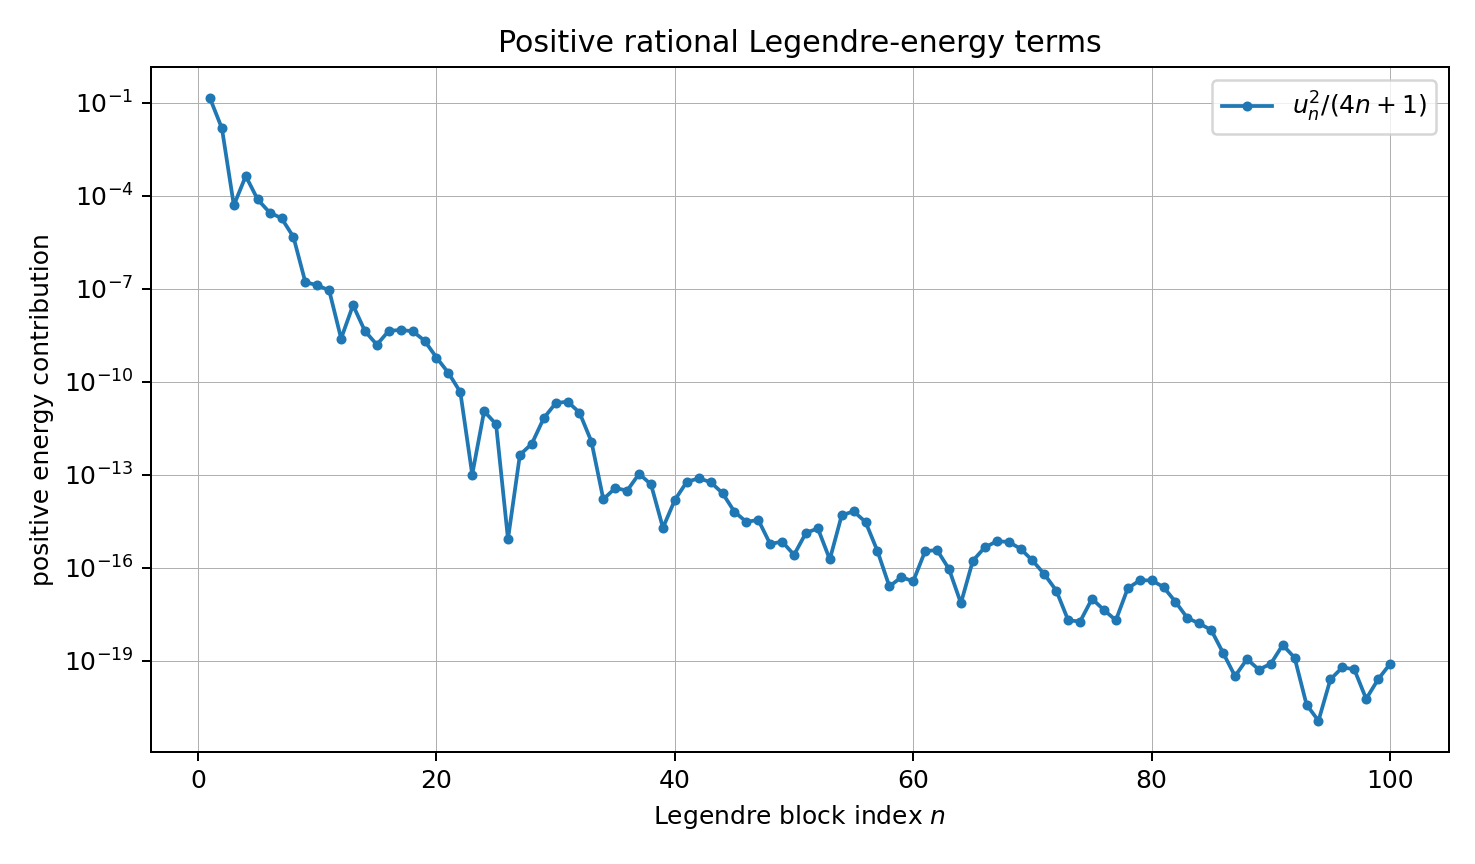
\includegraphics[width=0.91\textwidth]{energy_terms.png}
\caption{Positive contributions $u_n^2/(4n+1)$ on a logarithmic scale.}
\label{fig:energy-terms}
\end{figure}

\subsection{A nested dyadic-Fabius square series}

Let
\begin{equation}
 R_n:=\sum_{j=0}^{n}(-1)^{n+j}
 \binom{2n}{n+j}\binom{2n+2j}{2n}(2j)!
 2^{\binom{2j+1}{2}}F(2^{-2j-1}).
 \label{eq:Rn}
\end{equation}
Then $u_n=4^{-n}(4n+1)R_n$, and
\cref{thm:A2-series} immediately gives
\begin{equation}
 \boxed{
 A_2=\sum_{n=0}^{\infty}(4n+1)16^{-n}R_n^2.}
 \label{eq:A2-dyadic-square}
\end{equation}
Every summand is the square of a finite rational combination of dyadic Fabius
values.  Substituting any of the repository's q-binomial or Thue--Morse
formulas for those values turns \eqref{eq:A2-dyadic-square} into a completely
finite-inside-infinite q-arithmetic series.

\begin{problem}[Arithmetic of the square energy]
\label{prob:A2-arithmetic}
Determine whether $A_2$ is irrational or transcendental, and whether the three
representations \eqref{eq:A2-legendre}--\eqref{eq:A2-sinc} admit effective
Diophantine approximations stronger than their obvious rational partial sums.
The positivity of \eqref{eq:A2-legendre} is potentially useful because it
eliminates cancellation from the approximation error.
\end{problem}

\section{Sturm--Liouville and Sobolev energy hierarchies}
\label{sec:sturm}

Let
\begin{equation}
 \mathcal Lf=-\frac{\dd}{\dd x}\left((1-x^2)f'(x)\right).
 \label{eq:legendre-operator}
\end{equation}
Then
\begin{equation}
 \mathcal LP_{2n}=\lambda_nP_{2n},
 \qquad
 \lambda_n=2n(2n+1).
 \label{eq:eigenvalues}
\end{equation}
The endpoint factor $1-x^2$ makes integration by parts compatible with the
natural Legendre boundary condition.

\begin{theorem}[Orthogonal derivative energies; new here]
\label{thm:derivative-energies}
For $n,m\ge0$,
\begin{equation}
 \int_{-1}^{1}(1-x^2)B_n'(x)B_m'(x)\dd x
 =\delta_{nm}\lambda_n\frac{2u_n^2}{4n+1}.
 \label{eq:block-derivative-orthogonality}
\end{equation}
More generally, for every real $s\ge0$ for which the spectral norm is defined,
\begin{equation}
 \boxed{
 \norm{(I+\mathcal L)^{s/2}u}_2^2
 =\sum_{n=0}^{\infty}(1+\lambda_n)^s
 \frac{2u_n^2}{4n+1}.}
 \label{eq:spectral-sobolev}
\end{equation}
In particular,
\begin{equation}
 \int_{-1}^{1}(1-x^2)|u'(x)|^2\dd x
 =\sum_{n=0}^{\infty}\lambda_n\frac{2u_n^2}{4n+1}.
 \label{eq:first-derivative-energy}
\end{equation}
\end{theorem}

\begin{proof}
Use $B_n=u_nP_{2n}$ and self-adjointness:
\[
 \int(1-x^2)B_n'B_m'=\inner{\mathcal LB_n}{B_m}
 =\lambda_n\inner{B_n}{B_m}.
\]
Now apply \cref{thm:block-orthogonality}.  Equation
\eqref{eq:spectral-sobolev} is the spectral theorem for the nonnegative
self-adjoint Legendre operator, and \eqref{eq:first-derivative-energy} is its
$s=1$ quadratic-form part after subtracting \eqref{eq:parseval-up}.
\end{proof}

Because $u$ is $C^\infty$ and flat at the endpoints, all integer levels of
this hierarchy are finite.  The formulas therefore give infinitely many
positive series built from the same rational coefficients $u_n$, weighted by
explicit polynomial eigenvalues.  Their partial sums are rational and
monotone, providing convenient certified lower bounds for weighted derivative
energies.

\section{Nested grids, exact null trains, and a lifting law}
\label{sec:nested}

\subsection{A general interlevel null relation}

For an admissible lattice $m$, define the finite synthesis operator
\begin{equation}
 (T_mc)(x):=\sum_{|k|<2m}c_k u(x-k/m),
 \qquad -1\le x\le1.
 \label{eq:Tm}
\end{equation}
If $p$ is a polynomial and $Q=\Dscr p$, its canonical coefficient vector is
\begin{equation}
 (F_mp)_k:=\frac1mQ(k/m).
 \label{eq:Fm}
\end{equation}
Then \cref{thm:generic-synthesis} says $T_mF_mp=p$.

\begin{theorem}[Interlevel polynomial null train; new here]
\label{thm:interlevel-null}
Let $p$ have degree at most $d$, put $Q=\Dscr p$, and suppose both $m$ and
$rm$ are admissible, i.e. $\vtwo(m),\vtwo(rm)\ge d$.  Then
\begin{equation}
 \boxed{
 \frac1{rm}\sum_{|k|<2rm}
 \bigl(1-r\one_{r\mid k}\bigr)
 Q(k/(rm))u(x-k/(rm))=0}
 \label{eq:interlevel-null}
\end{equation}
for every $x\in[-1,1]$.
\end{theorem}

\begin{proof}
The fine representation is
\[
 p(x)=\frac1{rm}\sum_{|k|<2rm}Q(k/(rm))u(x-k/(rm)).
\]
Rewrite the coarse representation on the fine index set by setting $k=rj$:
\[
 p(x)=\frac r{rm}\sum_{\substack{|k|<2rm\\r\mid k}}
 Q(k/(rm))u(x-k/(rm)).
\]
Subtract the two identities.
\end{proof}

For the even Legendre hierarchy, take $m=m_n=4^n$ and $r=4$:
\begin{equation}
 \sum_{|k|<8m_n}
 \bigl(1-4\one_{4\mid k}\bigr)
 Q(k/(4m_n))u(x-k/(4m_n))=0.
 \label{eq:quarter-null}
\end{equation}
This is an explicit vector in the local kernel of the fine-grid synthesis
operator.  It is not obtained by solving a matrix nullspace: its entries are
samples of the same deconvolved polynomial, multiplied by the fixed mask
$1-4\one_{4\mid k}$.

\begin{figure}[H]
\centering
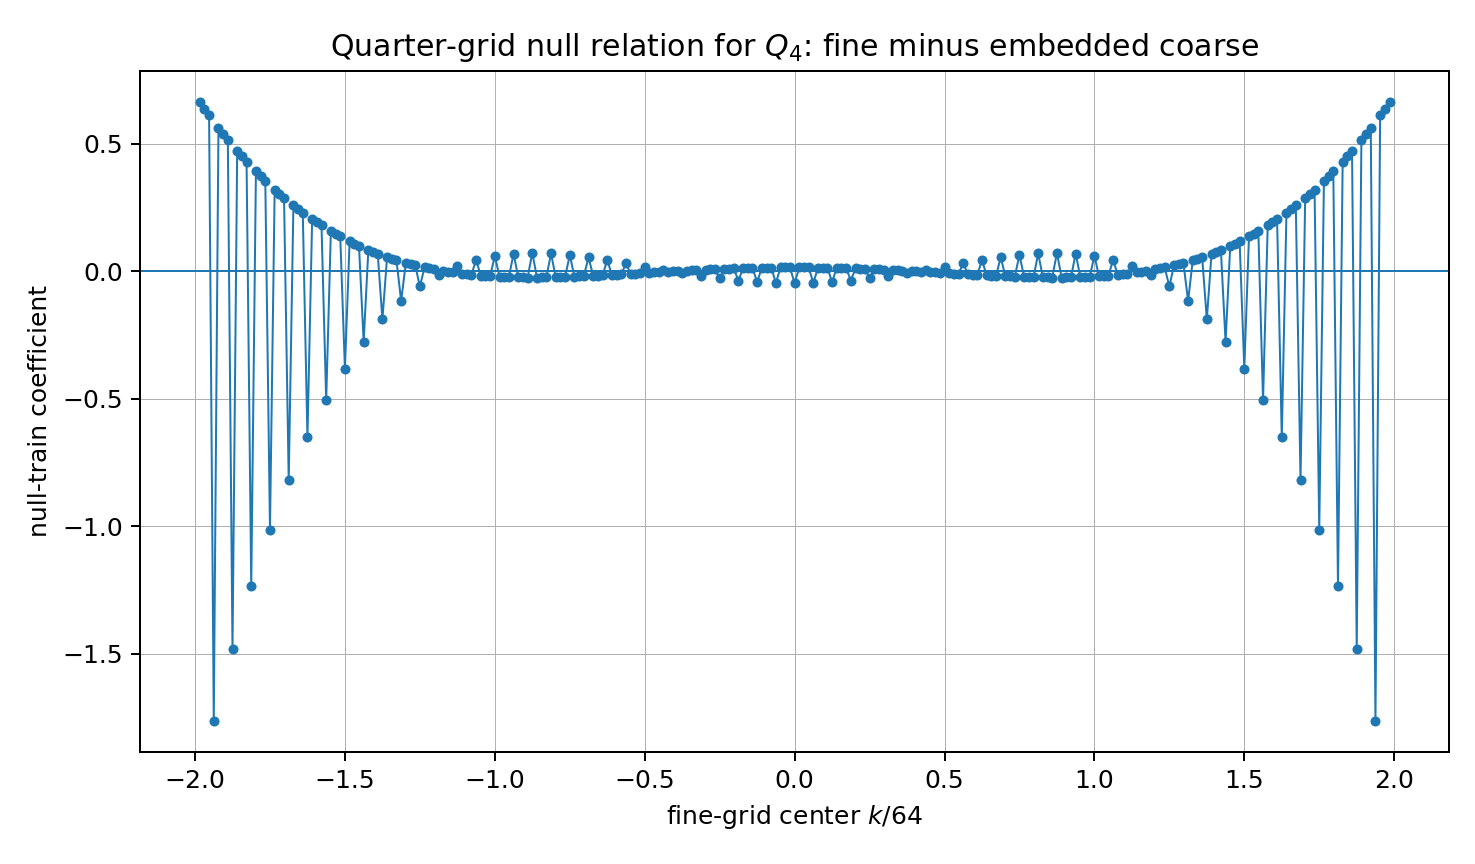
\includegraphics[width=0.92\textwidth]{quarter_grid_null_stencil.png}
\caption{The exact quarter-grid null coefficients for $Q_4$, comparing
$m=16$ with $m=64$.  The corresponding translate train vanishes identically
on $[-1,1]$ despite its substantial coefficients.}
\label{fig:quarter-null}
\end{figure}

\subsection{The refinement cocycle}

Let $E_r$ embed a coarse vector into the $r$-times finer grid:
\begin{equation}
 (E_rc)_k=
 \begin{cases}
 c_{k/r},&r\mid k,\\
 0,&r\nmid k.
 \end{cases}
 \label{eq:embedding}
\end{equation}
Then
\begin{equation}
 G_{m;r}p:=F_{rm}p-E_rF_mp
 \label{eq:gauge-vector}
\end{equation}
lies in $\ker T_{rm}$.  Refinements compose by the exact cocycle identity
\begin{equation}
 \boxed{
 G_{m;rs}p=G_{rm;s}p+E_sG_{m;r}p.}
 \label{eq:refinement-cocycle}
\end{equation}
Indeed, both sides telescope to $F_{rsm}p-E_sE_rF_mp$.  Thus all multilevel
null corrections can be built from one-step corrections without recomputing a
kernel basis.

\subsection{A quarter-grid lifting decomposition}

Let $a^{(N)}$ be the canonical fixed-scale coefficient vector for $S_N$:
\begin{equation}
 a_k^{(N)}=\frac1{m_N}C_N(k/m_N),
 \qquad |k|<2m_N.
 \label{eq:aN}
\end{equation}
Embed it into level $N+1$ with $E_4$.  Since
$C_{N+1}=C_N+u_{N+1}Q_{2N+2}$, direct subtraction yields the following exact
law.

\begin{theorem}[Exact Legendre--Rvachev lifting step; new here]
\label{thm:lifting}
For $m=m_N$ and $|k|<8m$,
\begin{equation}
 \boxed{
 a_k^{(N+1)}-(E_4a^{(N)})_k
 =\frac{1-4\one_{4\mid k}}{4m}C_N(k/(4m))
 +\frac{u_{N+1}}{4m}Q_{2N+2}(k/(4m)).}
 \label{eq:lifting}
\end{equation}
The first term synthesizes the zero function on $[-1,1]$; the second
synthesizes exactly the new orthogonal detail $B_{N+1}=u_{N+1}P_{2N+2}$.
Consequently,
\begin{equation}
 T_{m_{N+1}}\bigl(a^{(N+1)}-E_4a^{(N)}\bigr)=B_{N+1}.
 \label{eq:lifting-function}
\end{equation}
\end{theorem}

\begin{proof}
At a fine-grid point $t=k/(4m)$,
\[
 a_k^{(N+1)}=\frac1{4m}
 \bigl(C_N(t)+u_{N+1}Q_{2N+2}(t)\bigr),
\]
whereas $(E_4a^{(N)})_k=4\one_{4\mid k}C_N(t)/(4m)$.
This proves \eqref{eq:lifting}.  The first term is
\cref{thm:interlevel-null} applied to $p=S_N$; the second is
\eqref{eq:even-P-synthesis} multiplied by $u_{N+1}$.
\end{proof}

This is analogous in form to a lifting scheme, but with a significant
qualification.  The gauge component is not a wavelet detail: it is exactly
invisible on the target interval.  The genuine detail is the orthogonal
Legendre mode.  Coefficient refinement therefore decomposes into
\[
 \text{new coefficients}
 =\text{embedded old coefficients}
 +\text{null-space gauge}
 +\text{orthogonal spectral detail}.
\]
The accompanying program verifies the complete $N=1\to2$ identity, both
coefficientwise and as a function, with exact rational residual zero.

\section{Endpoint, center, and derivative sum rules}
\label{sec:sum-rules}

The finite synthesis identity can be sampled or differentiated to produce
families of exact dyadic identities involving $u$ and its derivatives.

\begin{theorem}[Endpoint jet sum rules; new here]
\label{thm:endpoint-jets}
Let $d\ge0$, $m=2^d$, and $0\le r\le d$.  Then
\begin{equation}
 \boxed{
 \frac1m\sum_{k=1}^{2m-1}Q_d(k/m)
 u^{(r)}(1-k/m)
 =\frac1{2^r}\frac{(d+r)!}{r!(d-r)!}.}
 \label{eq:endpoint-jets}
\end{equation}
For $r>d$, the same left side is zero.  At the left endpoint the value is
$(-1)^{d+r}$ times the right-hand side.
\end{theorem}

\begin{proof}
Differentiate \eqref{eq:Pd-synthesis} $r$ times.  At $x=1$, all terms with
$k\le0$ vanish because their atom arguments are at or beyond the flat endpoint
$1$; the displayed range $1\le k\le2m-1$ is exactly the surviving support.
The classical endpoint derivative is
\[
 P_d^{(r)}(1)=2^{-r}\frac{(d+r)!}{r!(d-r)!}
\]
for $r\le d$, and zero afterward.  Parity gives the left endpoint.
\end{proof}

The case $r=0$ is particularly simple:
\begin{equation}
 \sum_{k=1}^{2m-1}Q_d(k/m)u(1-k/m)=m.
 \label{eq:endpoint-value-sum}
\end{equation}
All arguments are dyadic, so every term is rational; the same is true for all
endpoint-jet identities because derivatives of $u$ at dyadic points are
rational \cite{Arias1982}.

\begin{theorem}[Central-binomial dyadic sum rule; new here]
\label{thm:center-sum}
For $n\ge0$ and $m=4^n$,
\begin{equation}
 \boxed{
 Q_{2n}(0)+2\sum_{k=1}^{m-1}Q_{2n}(k/m)u(k/m)
 =(-1)^n\binom{2n}{n}.}
 \label{eq:center-sum}
\end{equation}
\end{theorem}

\begin{proof}
Evaluate \eqref{eq:even-P-synthesis} at $x=0$.  The $k=\pm m$ boundary terms
vanish, and parity of $Q_{2n}$ and $u$ pairs the remaining positive and
negative indices.  Finally,
\[
 mP_{2n}(0)=4^n(-1)^n\frac1{4^n}\binom{2n}{n}.
\]
\end{proof}

This identity is notable because the factorially large value $Q_{2n}(0)$ is
balanced by a finite rational dyadic sum to leave the merely exponential
central binomial coefficient.  It is a local, exact manifestation of the
cancellation that dominates the closed loop.

\subsection{Mode-wise biorthogonality}

Multiplying \eqref{eq:Pd-synthesis} by $P_j$ and integrating gives, for
$j\ge0$,
\begin{equation}
 \frac1{2^d}\sum_{|k|<2^{d+1}}Q_d(k/2^d)
 \int_{-1}^{1}u(x-k/2^d)P_j(x)\dd x
 =\delta_{dj}\frac{2}{2d+1}.
 \label{eq:mode-biorthogonality}
\end{equation}
Thus the sampled deconvolution row is biorthogonal, through the truncated
translate moments, to every Legendre mode.  Equation
\eqref{eq:atom-gram} is the corresponding block-to-block form after a second
synthesis is inserted.

\section{Even Christoffel--Darboux projectors as dual translate frames}
\label{sec:frames}

\subsection{The even projection kernel}

Define
\begin{equation}
 K_N^{\mathrm e}(x,y)
 =\sum_{n=0}^{N}\frac{4n+1}{2}P_{2n}(x)P_{2n}(y).
 \label{eq:even-kernel}
\end{equation}
It is the kernel of the orthogonal projector onto
\begin{equation}
 E_N=\Span\{P_0,P_2,\ldots,P_{2N}\}.
 \label{eq:EN}
\end{equation}
If $K_d$ denotes the full Christoffel--Darboux kernel through degree $d$, then
\begin{equation}
 K_N^{\mathrm e}(x,y)=\frac12\bigl(K_{2N}(x,y)+K_{2N}(x,-y)\bigr).
 \label{eq:even-CD}
\end{equation}
Deconvolve in the first variable:
\begin{equation}
 K_N^\sharp(t,y)=
 \sum_{n=0}^{N}\frac{4n+1}{2}Q_{2n}(t)P_{2n}(y).
 \label{eq:even-sharp-kernel}
\end{equation}

\begin{theorem}[Finite translate factorization of the even projector; specialized here]
\label{thm:projector-factorization}
Put $m=4^N$.  Then
\begin{equation}
 \boxed{
 K_N^{\mathrm e}(x,y)=\frac1m\sum_{|k|<2m}
 K_N^\sharp(k/m,y)u(x-k/m).}
 \label{eq:kernel-atomization}
\end{equation}
Consequently, if
\begin{equation}
 g_k(x)=u(x-k/m),
 \qquad
 \psi_k(y)=\frac1mK_N^\sharp(k/m,y),
 \label{eq:dual-families}
\end{equation}
then
\begin{equation}
 \boxed{
 (\PiE_Nf)(x)=\sum_{|k|<2m}g_k(x)\inner{f}{\psi_k}.}
 \label{eq:dual-frame-projector}
\end{equation}
\end{theorem}

\begin{proof}
For fixed $y$, the function $x\mapsto K_N^{\mathrm e}(x,y)$ has degree $2N$.
Its deconvolution is exactly $K_N^\sharp(\cdot,y)$, so
\cref{thm:generic-synthesis} gives \eqref{eq:kernel-atomization}.  Integrate
against $f(y)$ to obtain \eqref{eq:dual-frame-projector}.
\end{proof}

The atoms $g_k$ do not lie in $E_N$ individually, so this is not an ordinary
basis expansion of the polynomial subspace.  It is a finite synthesis-analysis
factorization of its orthogonal projector: the analysis functions $\psi_k$ are
even polynomials, while the synthesis functions are compactly supported
translates.

\begin{corollary}[Trace and Hilbert--Schmidt identities; new here]
\label{cor:trace-identities}
The families in \eqref{eq:dual-families} satisfy
\begin{align}
 \sum_{|k|<2m}\inner{\psi_k}{g_k}&=N+1,
 \label{eq:trace-identity}\\
 \sum_{|k|,|\ell|<2m}
 \inner{g_k}{g_\ell}\inner{\psi_k}{\psi_\ell}&=N+1.
 \label{eq:HS-identity}
\end{align}
All inner products are over $[-1,1]$.
\end{corollary}

\begin{proof}
Write \eqref{eq:dual-frame-projector} as
$\PiE_N=\sum_k g_k\otimes\psi_k$.  The trace of a rank-one operator
$g\otimes\psi$ is $\inner{\psi}{g}$, while
$\tr\PiE_N=\rank\PiE_N=N+1$, proving \eqref{eq:trace-identity}.  Expanding the
Hilbert--Schmidt norm gives the double sum in \eqref{eq:HS-identity}; an
orthogonal projector has squared Hilbert--Schmidt norm equal to its rank.
\end{proof}

These identities give exact global diagnostics for any numerical realization
of the projector.  Unlike pointwise collocation checks, they test the complete
interaction between the truncated translate Gram matrix and the deconvolved
Legendre analysis Gram matrix.

\section{Factorial deconvolution and a sharp central-coefficient law}
\label{sec:asymptotic}

\subsection{Imported asymptotic input}

Let
\begin{equation}
 C=\MM(\pi\ii)
 =\prod_{j=1}^{\infty}\frac{\sin(\pi/2^j)}{\pi/2^j}.
 \label{eq:C-constant}
\end{equation}
The nearest poles of $1/\MM$ are $\pm2\pi\ii$.  The recent repository loop
report derives
\begin{equation}
 Q_{2n}(0)=
 \frac{2(-1)^n}{C}\frac{(4n)!}{(2n)!(4\pi)^{2n}}
 \left(1+\frac{2\pi^2}{4n-1}+\bigO(n^{-2})\right).
 \label{eq:Q0-asymptotic}
\end{equation}
In particular,
\begin{equation}
 \abs{Q_{2n}(0)}^{1/(2n)}\sim\frac{2n}{\pi\e},
 \qquad
 \frac{\abs{Q_{2n}(0)}^{1/n}}{n^2}\to\frac{4}{\pi^2\e^2}.
 \label{eq:Q0-root}
\end{equation}
The same report proves that
\begin{equation}
 c_n^{(0)}:=\frac{u_nQ_{2n}(0)}{4^n}
 \label{eq:central-coefficient}
\end{equation}
is unbounded in absolute value, ruling out atomwise flattening.

\subsection{Legendre coefficients cannot decay geometrically}

\begin{lemma}[Sharp root obstruction from nonanalyticity; new here]
\label{lem:un-root}
The Legendre coefficients of $u$ satisfy
\begin{equation}
 \boxed{
 \limsup_{n\to\infty}|u_n|^{1/n}=1.}
 \label{eq:un-root}
\end{equation}
\end{lemma}

\begin{proof}
Absolute convergence implies $u_n\to0$, hence the limsup is at most one.
Suppose it were $L<1$.  Choose a Bernstein ellipse parameter $\rho>1$ with
$L\rho^2<1$, and then choose $q$ so that $L<q<\rho^{-2}$.  Eventually
$|u_n|\le q^n$.  On every compact subset of the interior of that ellipse, the
classical complex bounds for Legendre polynomials give
$|P_{2n}(z)|\le C_K\rho^{2n}$.  Hence $\sum u_nP_{2n}(z)$ converges locally
uniformly and defines a holomorphic extension of $u$ to a neighborhood of
$[-1,1]$.  This contradicts the nowhere-analyticity of the Fabius--Rvachev
function \cite{Fabius1966}.  Thus the limsup is one.
\end{proof}

\begin{theorem}[Sharp root-limsup of the repeated central atom; new here]
\label{thm:central-root}
For the coefficient \eqref{eq:central-coefficient},
\begin{equation}
 \boxed{
 \limsup_{n\to\infty}
 \frac{|c_n^{(0)}|^{1/n}}{n^2}=\frac1{\pi^2\e^2}.}
 \label{eq:central-root}
\end{equation}
If
\begin{equation}
 V_n:=\frac{|u_n|}{4^n}
 \sum_{|k|<2\cdot4^n}|Q_{2n}(k/4^n)|
 \label{eq:block-variation}
\end{equation}
is the raw coefficient variation of the $n$th block, then
\begin{equation}
 \limsup_{n\to\infty}\frac{V_n^{1/n}}{n^2}
 \ge\frac1{\pi^2\e^2}.
 \label{eq:variation-lower}
\end{equation}
\end{theorem}

\begin{proof}
From \eqref{eq:central-coefficient},
\[
 \frac{|c_n^{(0)}|^{1/n}}{n^2}
 =|u_n|^{1/n}
 \frac{|Q_{2n}(0)|^{1/n}}{4n^2}.
\]
The second factor tends to $(\pi^2\e^2)^{-1}$ by
\eqref{eq:Q0-root}; the first has limsup one by
\cref{lem:un-root}.  This proves \eqref{eq:central-root}.  Since the $k=0$
term occurs in the absolute sum defining $V_n$, $V_n\ge|c_n^{(0)}|$.
\end{proof}

The theorem is substantially stronger than mere unboundedness.  Along a
subsequence, the $n$th root of the repeated central coefficient grows like
$n^2/(\pi^2e^2)$.  Thus the canonical coefficient rows are superexponential
along a subsequence, while their synthesized functions have
$L^2$ norm
\begin{equation}
 \norm{B_n}_2=|u_n|\sqrt{\frac{2}{4n+1}}\longrightarrow0.
 \label{eq:block-small}
\end{equation}
The closed loop is therefore an extreme cancellation mechanism.

\begin{table}[H]
\centering
\small
\begin{tabular}{@{}rrrrr@{}}
\toprule
$n$ & atoms & $|u_n|$ & $V_n$ & $V_n/|u_n|$\\
\midrule
0 & 3 & $5.000\times10^{-1}$ & $1.500$ & $3.00$\\
2 & 63 & $3.667\times10^{-1}$ & $9.057$ & $24.7$\\
4 & 1023 & $8.573\times10^{-2}$ & $45.549$ & $531$\\
6 & 16383 & $2.679\times10^{-2}$ & $230.706$ & $8.61\times10^3$\\
8 & 262143 & $1.243\times10^{-2}$ & $7921.35$ & $6.37\times10^5$\\
9 & 1048575 & $2.446\times10^{-3}$ & $37572.4$ & $1.54\times10^7$\\
\bottomrule
\end{tabular}
\caption{Full-grid double-precision scans of the exact rational coefficient
polynomials.  The raw variation grows while the synthesized mode shrinks.}
\label{tab:variation}
\end{table}

\begin{figure}[H]
\centering
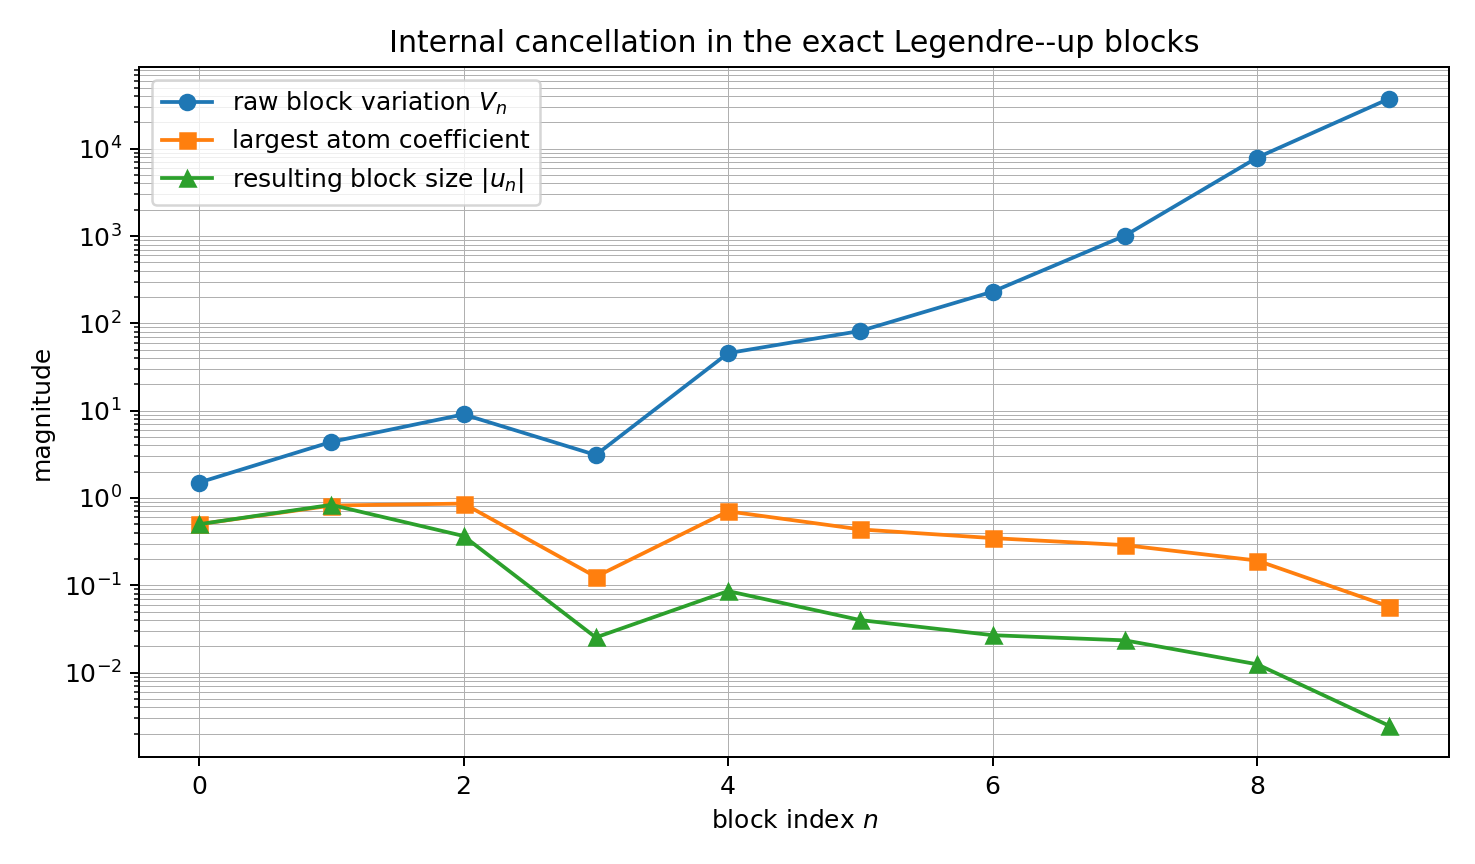
\includegraphics[width=0.92\textwidth]{block_cancellation_growth.png}
\caption{Internal coefficient variation, largest individual coefficient, and
resulting block size.  The rigorous asymptotic statement is
\eqref{eq:central-root}; the plot only illustrates the pre-asymptotic regime.}
\label{fig:cancellation}
\end{figure}

\subsection{\texorpdfstring{Lambert-$W$}{Lambert-W} threshold}

Solving the leading relation
$|Q_{2n}(0)|\asymp(2n/(\pi\e))^{2n}$ for the first index at which it exceeds
$X$ gives the imported threshold
\begin{equation}
 n_Q(X)=\frac{\log X}
 {2W\!\left(\log X/(\pi\e)\right)}+\bigO(1).
 \label{eq:Q-threshold}
\end{equation}
Here the principal branch $W$ appears because one inverts factorial growth.
This is distinct from the lower real branch $W_{-1}$ governing inversion of
the small-argument endpoint asymptotics of $F$.  The two occurrences share the
same algebraic core, inversion of a quantity of the form $y\log y$, but encode
different geometries.

\section{Connections across the Fabius--Rvachev corpus}
\label{sec:connections}

\subsection{Bell and Bernoulli polynomials}

The coefficient pipeline is
\[
 B_{2r}
 \longrightarrow \kappa_{2r}
 \longrightarrow \beta_{2r}
 \longrightarrow A_n(x)
 \longrightarrow Q_d(x)
 \longrightarrow Q_d(k/2^d).
\]
The first arrow is the dyadic cumulant factor
$(1-4^{-r})^{-1}$; the next two are complete Bell-polynomial transforms; the
last two are finite basis changes and dyadic sampling.  Bell and Bernoulli
polynomials therefore do not merely repackage the result: they are the exact
algebra that deconvolves the up probability law.

\subsection{q-binomial coefficients and dyadic arithmetic}

The coefficient $u_n$ is a finite transform of dyadic Fabius values by
\eqref{eq:un-dyadic}.  Those values have q-binomial and q-Pochhammer formulas in
the repository.  Substitution into \eqref{eq:A2-dyadic-square} creates a
positive outer series whose inner data are finite q-hypergeometric sums.  This
separates two roles:
\begin{itemize}
 \item q-binomial arithmetic computes the spectral weights $u_n$ exactly;
 \item the dyadic zero multiplicities of $\widehat u$ determine which sampled
 translate lattices reproduce the corresponding polynomial modes.
\end{itemize}
A useful future objective is to simplify their composition before squaring in
\eqref{eq:A2-dyadic-square}.

\subsection{Thue--Morse and nullspace geometry}

Thue--Morse signs appear in exact dyadic evaluation of $F$ and in the
annihilators used to compress active up-atoms.  The new interlevel relation
\eqref{eq:interlevel-null} is a different but compatible nullspace element: it
arises by subtracting two exact Poisson reproductions.  For dyadic refinement
$r=2^s$, its periodic mask $1-r\one_{r\mid k}$ should be compared with the
cyclotomic/q-integer factors
\begin{equation}
 \prod_{j=1}^{d}[2^j]_z,
 \qquad [N]_z=1+z+\cdots+z^{N-1},
 \label{eq:q-annihilator}
\end{equation}
that generate the repository's local polynomiality defects.  Their precise
factorization relationship is an open algebraic problem stated below.

\subsection{Infinite sinc products and energy}

The same product \eqref{eq:fourier-product} has three simultaneous meanings:
\begin{enumerate}
 \item it is the characteristic function of the random series
 \eqref{eq:random-series};
 \item its integer zero multiplicities create exact polynomial reproduction;
 \item its squared modulus integrates to the positive energy
 \eqref{eq:A2-sinc}.
\end{enumerate}
Thus the finite shifted-polynomial theorem and the global $L^2$ norm are not
separate phenomena.  Both are consequences of the same sinc product, one
through its zeros and the other through its magnitude.

\section{Numerical and exact verification}
\label{sec:verification}

\subsection{Exact arithmetic checks}

The accompanying script uses Python's arbitrary-precision integers and
\texttt{Fraction}.  Moments are generated from Bernoulli cumulants; reciprocal
MGF coefficients use an exact exponential-generating-function recurrence;
Legendre and deconvolved polynomials are manipulated coefficientwise; dyadic
values of $u$ are evaluated from the finite Thue--Morse/moment formula.

\begin{table}[H]
\centering
\small
\begin{tabular}{@{}rrrrr@{}}
\toprule
Degree $d$ & $m=2^d$ & atoms & dyadic test points & max exact residual\\
\midrule
0 & 1 & 3 & 9 & $0$\\
1 & 2 & 7 & 17 & $0$\\
2 & 4 & 15 & 17 & $0$\\
3 & 8 & 31 & 17 & $0$\\
4 & 16 & 63 & 17 & $0$\\
5 & 32 & 127 & 17 & $0$\\
6 & 64 & 255 & 17 & $0$\\
\bottomrule
\end{tabular}
\caption{Exact verification of \eqref{eq:Pd-synthesis}.}
\label{tab:exact-checks}
\end{table}

Two further checks return the rational number zero:
\begin{itemize}
 \item the complete $P_4$ quarter-grid null train $m=16\to64$ at seventeen
 dyadic points;
 \item the $N=1\to2$ lifting law, first coefficientwise and then as a function
 at seventeen dyadic points.
\end{itemize}
No floating approximation enters those tests.

\subsection{Reproduction command}

From the artifact directory, run
\begin{lstlisting}[style=pythonstyle]
python legendre_rvachev_experiments.py
\end{lstlisting}
The program regenerates all CSV files and figures.  Useful options are
\begin{lstlisting}[style=pythonstyle]
python legendre_rvachev_experiments.py --no-plots
python legendre_rvachev_experiments.py --max-spectral-mode 120
\end{lstlisting}
The full-grid coefficient scan is floating point because the $n=9$ block
already contains $1{,}048{,}575$ atoms; its polynomial and spectral
coefficients are nevertheless generated exactly before conversion.

\section{Conjectures and frontier directions}
\label{sec:frontiers}

\begin{conjecture}[Legendre coefficient saddle law]
\label{conj:legendre-saddle}
Away from a possible sparse set of near-cancellation indices, the coefficients
$u_n$ obey a dyadic saddle asymptotic of the form
\begin{equation}
 \log|u_n|=-\frac{(\log n)^2}{2\log2}
 +\bigO(\log n\log\log n),
 \label{eq:legendre-saddle-conj}
\end{equation}
with a bounded or slowly varying log-periodic correction inherited from the
binary endpoint phase of $F$.
\end{conjecture}

The same quadratic-log scale occurs in the Fourier-decay and endpoint
asymptotic parts of the corpus.  A proof should combine a Hilb or Debye
approximation for $P_{2n}$ with the lower-branch Lambert-$W$ expansion of the
flat endpoint layer.  It would turn the root-limsup theorem
\eqref{eq:central-root} into a full asymptotic for the canonical central atom.

\begin{conjecture}[Exterior side-lobe explosion]
\label{conj:side-lobes}
Extend the finite train $B_n$ from \eqref{eq:block-def} to all of $\R$ by the
same formula and call it $\widetilde B_n$.  Although
$\widetilde B_n=u_nP_{2n}$ on $[-1,1]$, conjecturally
\begin{equation}
 \frac{\norm{\widetilde B_n}_{L^2(\R\setminus[-1,1])}}
 {\norm{B_n}_{L^2[-1,1]}}\longrightarrow\infty.
 \label{eq:side-lobe-conj}
\end{equation}
A stronger version predicts superexponential growth along a subsequence.
\end{conjecture}

This would make the local nature of exact polynomial reproduction visible in
physical space: enormous exterior side lobes would cancel only on the target
interval.

\begin{problem}[Optimal null-space gauge]
\label{prob:gauge}
At a fixed fine scale, add arbitrary vectors from the complete dyadic alias
nullspace to the canonical sampled coefficient row.  Determine the unique
minimum-$\ell^2$ row, the minimum-$\ell^1$ variation, and their asymptotics for
$P_{2n}$ and $S_N$.  Can a multilevel choice of gauges make the lifting updates
numerically stable without destroying exactness?
\end{problem}

The root-limsup theorem applies to the canonical sampled gauge.  Whether every
exact literal-shift representation must exhibit comparable growth is a deeper
question about the smallest singular values of the local synthesis map.

\begin{problem}[Cyclotomic factorization of refinement nulls]
\label{prob:cyclotomic-null}
Express the coefficient sequence in \eqref{eq:interlevel-null}, for
$r=2^s$, in the repository's q-integer/Thue--Morse nullspace basis.  Determine
whether the refinement cocycle \eqref{eq:refinement-cocycle} corresponds to a
factorization or filtration of
$\prod_{j=1}^{d}[2^j]_z$ by cyclotomic shells.
\end{problem}

\begin{problem}[Tight or well-conditioned projector frames]
\label{prob:tight-frame}
The dual families $g_k,\psi_k$ in \eqref{eq:dual-families} factor an
orthogonal projector but are highly redundant and poorly conditioned.  Find a
nullspace gauge, a nonuniform subset of centers, or a weighted inner product in
which the same exact projector has near-tight frame bounds.  The trace and
Hilbert--Schmidt identities \eqref{eq:trace-identity}--\eqref{eq:HS-identity}
provide invariant constraints for this optimization.
\end{problem}

\begin{conjecture}[Irrationality of the Fabius square energy]
\label{conj:A2-irrational}
The constant
\(
 A_2=\int_0^1F(x)^2\dd x
\)
is irrational.
\end{conjecture}

Even this first arithmetic classification appears nontrivial.  The positive
rational series, sinc-product integral, and dyadic-Fabius square series supply
three very different starting points; transcendence is a natural stronger
question only after irrationality is understood.

\subsection{Higher-dimensional and other orthogonal systems}

The logical pattern is not specific to Legendre polynomials.  Whenever a
compactly supported atom reproduces a polynomial space and a target function
has an orthogonal polynomial expansion, every spectral mode can be replaced by
a finite atom train.  What is special here is the simultaneous exactness of
all arithmetic ingredients: rational moments, dyadic zero multiplicities,
Bell--Bernoulli deconvolution, and compact support.  Promising extensions are:
\begin{itemize}
 \item Jacobi and Gegenbauer systems, with endpoint weights chosen to match
 differentiated energy forms;
 \item tensor-product and box-spline analogues of the recent multivariate
 up-like constructions \cite{CharinaContiDyn2024};
 \item spherical harmonics combined with radial compactly supported atoms;
 \item nonstationary subdivision atoms whose zero multiplicities grow by a
 prescribed arithmetic schedule.
\end{itemize}

\section{Formalization roadmap}
\label{sec:formalization}

The new results divide naturally into finite algebra and standard Hilbert-space
arguments.

\begin{enumerate}
 \item \textbf{Polynomial layer.}  At compiled checkpoint \texttt{a3854643d},
 \path{RvachevMomentAppell.lean} formalizes the full rational raw moments,
 their formal reciprocal/Bell sequence, the rational and real monic
 reciprocal-moment Appell families, and coefficientwise polynomial
 deconvolution with exact smoothing recovery and exact preservation of the
 original top coefficient, natural degree, and leading coefficient.  The same
 checkpoint packages
 deconvolution as a real linear map, proves its zero, addition, scalar,
 finite-sum, and constant-multiple laws, and identifies its values on monomials
 and $X^n$; it also proves the kernel is trivial and both the linear and raw
 operations are injective.
 The analytic reciprocal-MGF/differential-series display, specialized parity,
 explicit low coefficients, and a specialized reciprocal recurrence remain
 outside that API.
 \item \textbf{Synthesis and Legendre specialization.}  At compiled checkpoint
 \texttt{a3854643d}, \path{RvachevPolynomialSynthesis.lean} formalizes the
 global and finite sufficient-mesh forms of \eqref{eq:generic-synthesis}, and
 \path{FabiusLegendreTranslateBlocks.lean} packages \eqref{eq:Pd-synthesis}
 and \eqref{eq:even-P-synthesis} at meshes $2^d$ and $4^n$, together with
 exact degree $d$ and leading coefficient $2^{-d}\binom{2d}{d}$ for $Q_d$.
 The focused-build \path{CompositeMeshSharpness.lean} now proves the sharp
 classification and least natural mesh for universal exactness on the entire
 degree-$d$ space, including the $4^N$ specialization for the whole space
 through degree $2N$.  Minimality for an individual $P_d$, block, or $S_N$ and
 the closed derivative/Gegenbauer/Appell forms of $Q_d$ remain targets.
 \item \textbf{Orthogonal block layer.}  Complete orthogonality of the
 polynomial-form blocks, the coefficient Parseval identity, and the exact tail
 are formalized in \path{FabiusLegendreEnergy.lean}.  The same checkpoint's
 \path{FabiusLegendreTranslateBlocks.lean} now formalizes the literal finite
 up-translate realization, its complete block orthogonality, and the atom-Gram
 formula.  At compiled checkpoint \texttt{a3854643d}, the focused-build
 \path{FabiusLegendreTranslateSeries.lean} now
 formalizes pointwise and uniform absolute summability and
 \texttt{HasSum}/\texttt{tsum} forms for the literal outer blocks, the finite
 mode expansion of $C_N=\Dscr S_N$, both global and finite common-mesh
 synthesis at $4^N$, and convergence of the common-mesh partial trains to $u$
 in $C([-1,1])$, with raw uniform, norm-error, and pointwise forms.  Rationality
 of those atom rows, equality of the two
 coefficient vectors, an unconditional $\operatorname{natDegree}(S_N)=2N$
 statement, and nonvanishing of the top Legendre coefficient remain outside
 these APIs; the natural degree and leading coefficient of $C_N$ are proved equal to
 those of $S_N$, including degenerate drops.
 \item \textbf{Energy layer.}  The real-variable equality
 \eqref{eq:A2-legendre} is formalized in \path{FabiusLegendreEnergy.lean}.
 At checkpoint \texttt{9d5f41c2c},
 \path{FabiusLegendreRationalEnergy.lean} also formalizes its positive rational
 monotone partial sums, convergence of their real casts to $A_2$, and all four
 exact values in \eqref{eq:A2-first}.  At checkpoint \texttt{b9b240bc0},
 \path{FabiusSquareEnergyFourier.lean} formalizes the full and positive-half-line
 Fourier energies and closes \eqref{eq:A2-fourier}--\eqref{eq:A2-sinc} with its
 four-theorem API.
 \item \textbf{Refinement layer.}  Define finite index embeddings $E_r$ and
 prove \eqref{eq:interlevel-null} by subtraction.  The lifting theorem then
 reduces to coefficient normalization and linearity.
 \item \textbf{Endpoint layer.}  Differentiate the finite sum, use flat support
 at $\pm1$, and import the closed endpoint derivatives of $P_d$.
 \item \textbf{Projector layer.}  Formalize finite-rank operators
 $g\otimes\psi$, traces, and Hilbert--Schmidt norms to obtain
 \cref{cor:trace-identities}.
 \item \textbf{Asymptotic layer.}  Reuse the existing theorem for
 $Q_{2n}(0)$; prove that geometric Legendre decay yields analytic extension;
 conclude the root-limsup law \eqref{eq:central-root}.
\end{enumerate}

The orthogonal block theorem is now formalized in \path{FabiusLegendreEnergy.lean}
and \path{FabiusLegendreTranslateBlocks.lean}; only the interlevel identities remain
as a relatively short formalization target because their analytic content is already
isolated in existing repository theorems.  The only new complex-analytic lemma needed
for the sharp central law is the standard implication from geometric Legendre coefficient decay to holomorphic extension in a Bernstein ellipse.

\section{Conclusion}
\label{sec:conclusion}

The requested finite representation is completely explicit.  For degree $d$,
one applies the reciprocal moment operator $\Dscr=\MM(D)^{-1}$ to $P_d$,
samples the resulting polynomial $Q_d$ at the grid $2^{-d}\Z$, and attaches
those samples to finitely many literal translates of $u$.  For the even modes
in the canonical expansion, the grids are $4^{-n}\Z$ and nest by quarter-grid
refinement.

Substitution closes the loop exactly, but its correct unit is a finite
cancellation block.  The new orthogonality theorem shows that these blocks are
not arbitrary: they are a complete orthogonal resolution of $u$ in
$L^2[-1,1]$.  This yields exact tails, atom-Gram identities, rank-one detail
projectors, and an infinite hierarchy of positive spectral energies.  The
simplest energy is the square integral of the Fabius function, simultaneously
a positive rational Legendre series and an infinite sinc-product integral.

The nested grids introduce a second structure.  Refining an exact polynomial
coefficient row adds a computable null train.  Refining a Legendre partial sum
adds that invisible gauge correction plus precisely one new orthogonal mode.
This is an exact lifting law rather than a numerical analogy.

Finally, the loop is intrinsically ill-conditioned in its canonical atom
coordinates.  Factorial moment deconvolution combines with the absence of any
geometric Legendre decay to force the repeated central coefficient to have
root-limsup $n^2/(\pi^2e^2)$.  The function-level series is exceptionally
well behaved; the atom-level flattening is exceptionally badly behaved.  Any
stable computational realization must therefore preserve the spectral block
structure, exploit nullspace gauges, or redesign the dictionary rather than
merely reorder the individual translates.

\appendix

\section{Exact recurrences used by the program}
\label{app:recurrences}

The moments satisfy the cumulant recurrence
\begin{equation}
 \mu_0=1,
 \qquad
 \mu_n=\sum_{j=1}^{n}\binom{n-1}{j-1}\kappa_j\mu_{n-j}.
 \label{eq:moment-recurrence}
\end{equation}
The reciprocal-MGF coefficients satisfy
\begin{equation}
 \beta_0=1,
 \qquad
 \beta_n=-\sum_{j=1}^{n}\binom{n}{j}\mu_j\beta_{n-j}.
 \label{eq:beta-recurrence}
\end{equation}
The Legendre recurrence is
\begin{equation}
 (d+1)P_{d+1}(x)=(2d+1)xP_d(x)-dP_{d-1}(x).
 \label{eq:legendre-recurrence}
\end{equation}
After each $P_d$ is constructed, the finite operator
\eqref{eq:deconvolution} produces $Q_d$, and
\eqref{eq:un-moments} produces $u_n$.

For exact dyadic verification, the program uses, for integers $n\ge0$ and
$0\le a\le2^n$, the finite formula
\begin{equation}
 F(a/2^n)=\frac{2^{-n(n+1)/2}}{n!}
 \sum_{j=0}^{a-1}(-1)^{s_2(j)}
 \sum_{r=0}^{\floor{n/2}}
 \binom{n}{2r}\mu_{2r}(2a-2j-1)^{n-2r},
 \label{eq:dyadic-F}
\end{equation}
where $s_2(j)$ is the binary digit sum.  Then
\begin{equation}
 u(q/2^n)=F(1-|q|/2^n)
 \label{eq:dyadic-up}
\end{equation}
inside the support and is zero at or beyond its endpoints.

\section{Artifact inventory}
\label{app:inventory}

The accompanying ZIP archive contains:
\begin{itemize}
 \item \texttt{legendre\_rvachev\_self\_reconstruction.tex} and its compiled
 PDF;
 \item \texttt{legendre\_rvachev\_experiments.py}, fully commented and
 executable offline;
 \item \texttt{README.txt} with reproduction instructions;
 \item \texttt{CORPUS\_AUDIT.md}, \texttt{REPOSITORY\_SNAPSHOT.txt}, and
 \texttt{SHA256SUMS.txt} documenting provenance and package integrity;
 \item exact CSV checks for Legendre synthesis, the quarter-grid null train,
 and the lifting step;
 \item exact Legendre/deconvolution coefficients and positive rational energy
 partial sums;
 \item the full-grid coefficient-conditioning table;
 \item all PDF and PNG figures used in the report.
\end{itemize}

\begin{thebibliography}{99}

\bibitem{Fabius1966}
J.~Fabius,
\newblock A probabilistic example of a nowhere analytic $C^\infty$-function,
\newblock \emph{Zeitschrift f\"ur Wahrscheinlichkeitstheorie und Verwandte
Gebiete} \textbf{5} (1966), 173--174.

\bibitem{Rvachev1971}
V.~L.~Rvachev and V.~A.~Rvachev,
\newblock A certain finite function,
\newblock \emph{Dopovidi Akademii Nauk Ukrains'koi RSR, Series A} (1971),
705--707, 764.

\bibitem{Rvachev1972}
V.~L.~Rvachev and V.~A.~Rvachev,
\newblock On the representation of polynomials by functions with compact
support,
\newblock in \emph{Mathematical Physics}, No.~11, Naukova Dumka, Kiev, 1972,
126--129.

\bibitem{Arias1982}
J.~Arias de Reyna,
\newblock An infinitely differentiable function with compact support:
definition and properties,
\newblock English translation of \emph{Rev. Real Acad. Ciencias Madrid}
\textbf{76} (1982), 21--38; arXiv:1702.05442 (2017).

\bibitem{AriasArithmetic}
J.~Arias de Reyna,
\newblock Arithmetic of the Fabius function,
\newblock \emph{INTEGERS} \textbf{18} (2018), Article A51;
arXiv:1702.06487.

\bibitem{Have2017}
S.~G.~Have,
\newblock A recurrence relation for the odd order moments of the Fabius
function,
\newblock arXiv:1703.01904 (2017).

\bibitem{StrangFix1973}
G.~Strang and G.~Fix,
\newblock A Fourier analysis of the finite element variational method,
\newblock in \emph{Constructive Aspects of Functional Analysis}, C.I.M.E.,
1973, 793--840.

\bibitem{Szego1975}
G.~Szeg\H{o},
\newblock \emph{Orthogonal Polynomials}, 4th ed.,
\newblock American Mathematical Society Colloquium Publications, Vol.~23,
1975.

\bibitem{Roman1984}
S.~Roman,
\newblock \emph{The Umbral Calculus},
\newblock Academic Press, 1984.

\bibitem{Comtet1974}
L.~Comtet,
\newblock \emph{Advanced Combinatorics},
\newblock Reidel, 1974.

\bibitem{AlloucheShallit2003}
J.-P.~Allouche and J.~Shallit,
\newblock \emph{Automatic Sequences: Theory, Applications, Generalizations},
\newblock Cambridge University Press, 2003.

\bibitem{CharinaContiDyn2024}
M.~Charina, C.~Conti, and N.~Dyn,
\newblock Multivariate compactly supported $C^\infty$ functions by subdivision,
\newblock \emph{Applied and Computational Harmonic Analysis} \textbf{70}
(2024), 101630; arXiv:2211.05677.

\bibitem{ProveItPrimary}
V.~Reshetnikov,
\newblock \emph{The Fabius Function and Rvachev's Up-Function},
\newblock primary exposition in the \texttt{ProveIt} repository,
\repo, snapshot \texttt{faa3a9b94ac0e71abdc53c36fdf428222e4d2a8c},
29 August 2026.

\bibitem{ProveItSynthesis}
V.~Reshetnikov,
\newblock \emph{Exact Polynomial Synthesis from Rvachev Up-Atoms},
\newblock consolidated frontier volume under
\nolinkurl{semi-formalized-research-frontiers/drafts/representations/Up_Polynomial_Synthesis/},
2026.

\bibitem{ProveItLoopV3}
V.~Reshetnikov,
\newblock \emph{Closing the Lagrange--Legendre--Rvachev Loop},
\newblock report under
\nolinkurl{semi-formalized-research-frontiers/drafts/representations/lagrange_rvachev_loop_report_v3/},
2026.

\bibitem{ProveItLoopV5}
V.~Reshetnikov,
\newblock \emph{Closing the Rvachev--Lagrange Loop: Exact Fixed-Radius
Up-Function Synthesis of Lagrange Polynomials and Coefficient-Space
Projectors},
\newblock report under
\nolinkurl{semi-formalized-research-frontiers/drafts/representations/Rvachev_Lagrange_Loop_Report_v5/},
2026.

\end{thebibliography}

\end{document}
